\label{ch:appendixA}

This appendix compiles all the cases simulated in this study as part of a sanity check to ensure that the solver works properly. Some of these cases were verified using other solvers, while others are simulations without comparison.

\section{2D C3 Benchmark}

The C3 reactor benchmark is a case for heterogeneous system. It is based on the C3 benchmark on deterministic transport calculations \cite{cavarecOECDNEABenchmark1994} and it is perturbed by introducing a localized neutron noise source. The system configuration is given in Figure \ref{fig:C3_configuration}. It consists of two UO2 fuel assemblies (at North-West and South-East positions) and two MOX fuel assemblies (at North-East and South-West positions). The size of each fuel assembly is 21.42 cm x 21.42 cm. The dark blue squares in the illustration are guide tubes; the ones in the center of the fuel assemblies contain fission chambers. Reflective boundary conditions are imposed. The perturbation is a fluctuation of 5\% of the fast and thermal neutron capture cross-sections in the fuel cell (16,19) identified with a red square in Figure \ref{fig:C3_configuration}.
\begin{figure}[H]
        \centering
        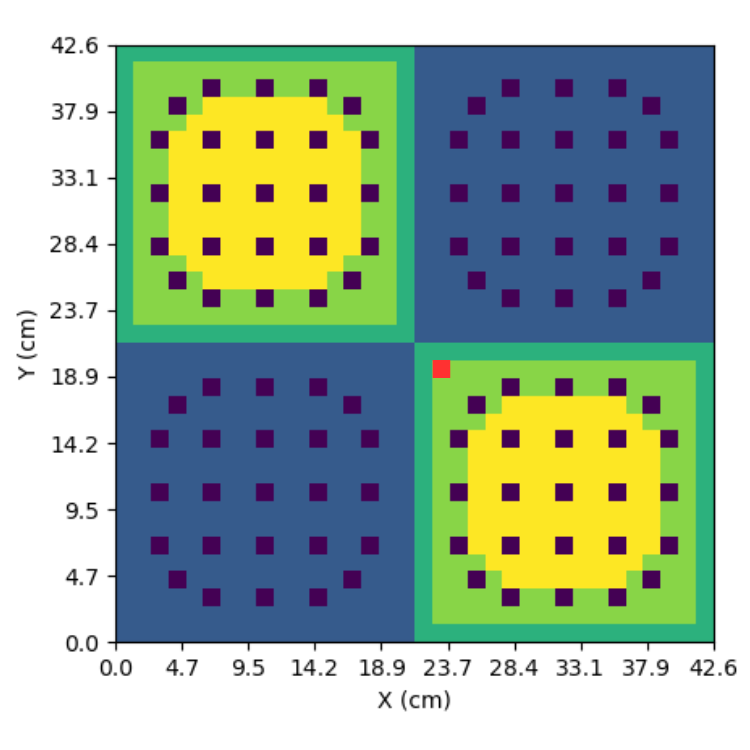
\includegraphics[width=0.6\textwidth]{figures/C3_configuration.png}
        \caption{Configuration of C3 Benchmark (obtained from \cite{mylonakisNeutronNoiseSimulations2019})}
        \label{fig:C3_configuration}
\end{figure}

For this simulation, CORE SIM+ results using finite difference are available. Therefore, the results from simulation will be compared to the CORE SIM+ results for forward flux, adjoint, and neutron noise calculation. The flux differences are calculated as relative error defined as follows:
\begin{equation}\label{eq:error1}
    \varepsilon = \frac{|\phi_{\text{solver}} - \phi_{\text{ref}}|}{|\phi_{\text{ref}}|} \times 100\%
\end{equation}

\subsection{Forward Flux Solution}

The forward flux solutions from CORE SIM+, the developed solver, and comparison between the simulators are as follow:
\begin{table}[H]
        \centering
        \caption{Eigenvalue comparison of 2D C3 Benchmark}
        \label{table:C3_fw_results}
        \begin{tabular}{ | M{3.5cm} | M{2cm} | } 
         \hline
         $k_{\text{eff}}$ CORE SIM+ & 1.019060  \\
         \hline
         $k_{\text{eff}}$ solver & 1.019060  \\
         \hline
         Absolute Error (pcm) & 0.0  \\
         \hline
        \end{tabular}
\end{table}

\begin{figure}[H]
        \centering
        \begin{subfigure}{.48\textwidth}
          \centering
          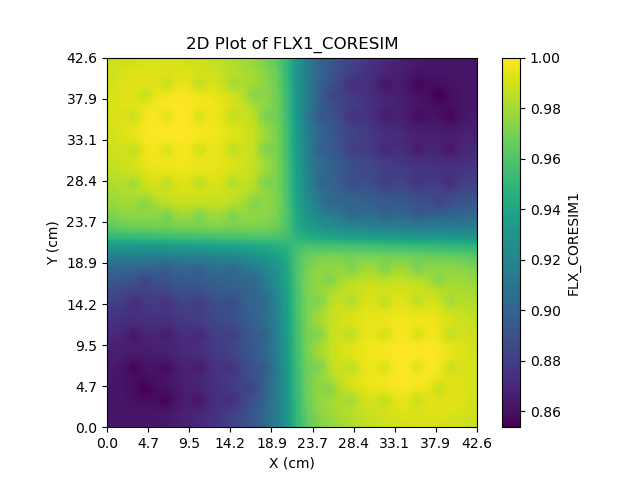
\includegraphics[width=\linewidth]{figures/OBJECTIVES1_TEST02_2DMG_C3_VandV_FORWARD_FLX_CORESIM_G1.png}
        \end{subfigure}
        \hfill
        \begin{subfigure}{.48\textwidth}
          \centering
          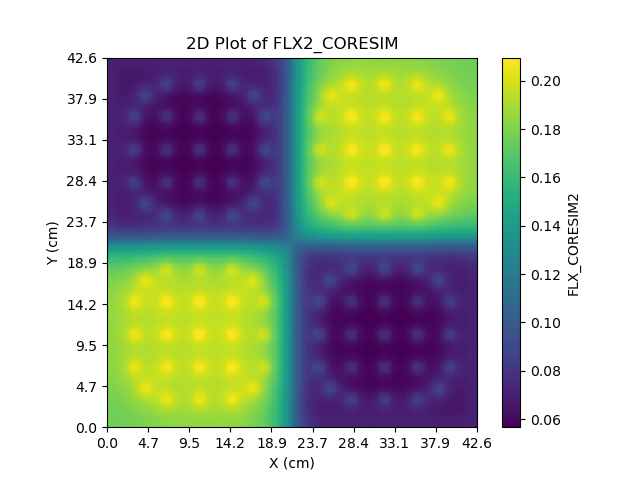
\includegraphics[width=\linewidth]{figures/OBJECTIVES1_TEST02_2DMG_C3_VandV_FORWARD_FLX_CORESIM_G2.png}
        \end{subfigure}
        \caption{Forward flux results from CORE SIM+}
        \label{fig:C3_fw_results_flx}
\end{figure}
\begin{figure}[H]
        \centering
        \begin{subfigure}{.48\textwidth}
          \centering
          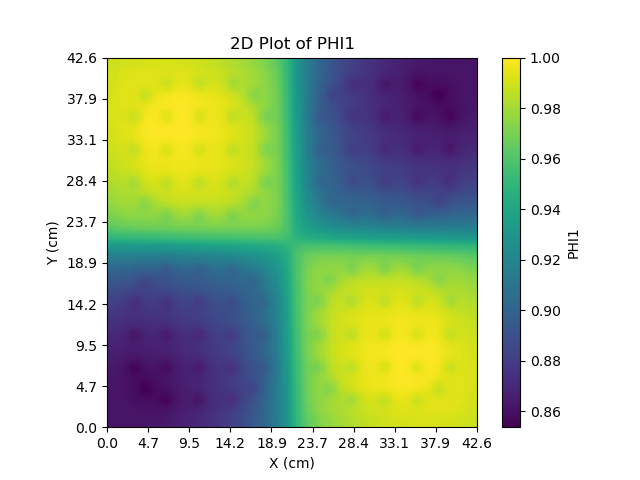
\includegraphics[width=\linewidth]{figures/OBJECTIVES1_TEST02_2DMG_C3_VandV_FORWARD_PHI_G1.png}
        \end{subfigure}
        \hfill
        \begin{subfigure}{.48\textwidth}
          \centering
          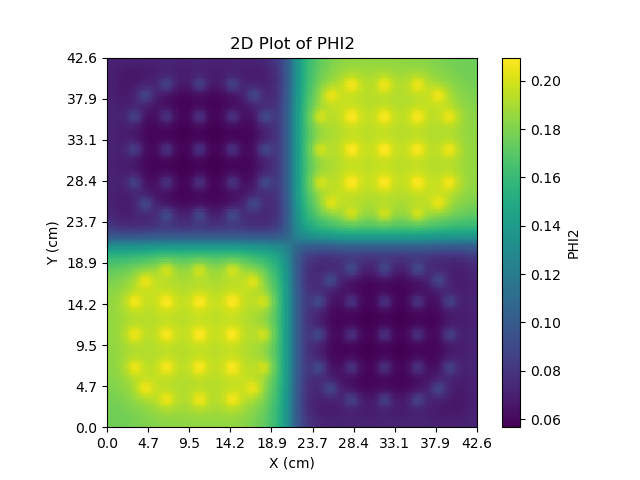
\includegraphics[width=\linewidth]{figures/OBJECTIVES1_TEST02_2DMG_C3_VandV_FORWARD_PHI_G2.png}
        \end{subfigure}
        \caption{Forward flux results from the developed solver}
        \label{fig:C3_fw_results_phi}
\end{figure}
\begin{figure}[H]
        \centering
        \begin{subfigure}{.48\textwidth}
          \centering
          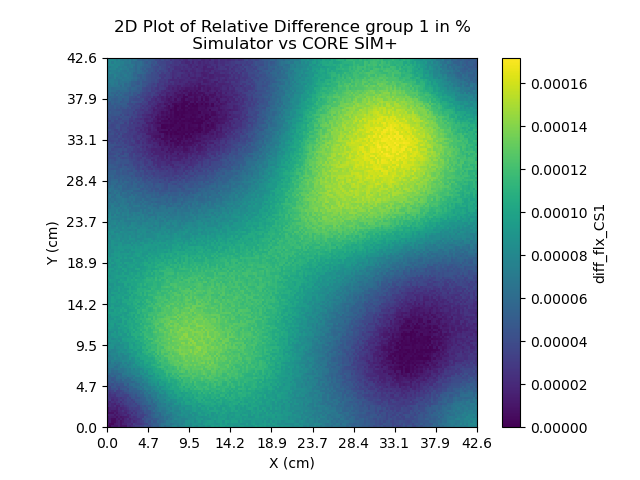
\includegraphics[width=\linewidth]{figures/OBJECTIVES1_TEST02_2DMG_C3_VandV_FORWARD_diff_flx_CS_G1.png}
        \end{subfigure}
        \hfill
        \begin{subfigure}{.48\textwidth}
          \centering
          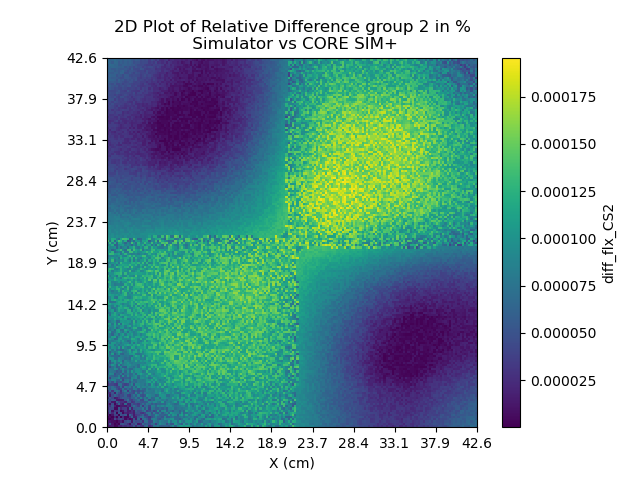
\includegraphics[width=\linewidth]{figures/OBJECTIVES1_TEST02_2DMG_C3_VandV_FORWARD_diff_flx_CS_G2.png}
        \end{subfigure}
        \caption{Difference of forward flux between CORE SIM+ and the solver}
        \label{fig:C3_fw_results_diff_phi}
\end{figure}

As seen in Table \ref{table:C3_fw_results}, Figure \ref{fig:C3_fw_results_flx}, Figure \ref{fig:C3_fw_results_phi}, and Figure \ref{fig:C3_fw_results_diff_phi}, the results show that the solver agrees well with CORE SIM+. The $k_{\text{eff}}$ matches between CORE SIM+ and solver exactly. This is due to the fact that this solver uses similar discretization to CORE SIM+. The error is less than 1\% for the forward flux. This shows that the solver works well for 2D rectangular geometries.

\subsection{Adjoint Flux Solution}

The adjoint flux solutions from CORE SIM+, the developed solver, and comparison between the simulators are as follows:
\begin{figure}[H]
        \centering
        \begin{subfigure}{.48\textwidth}
          \centering
          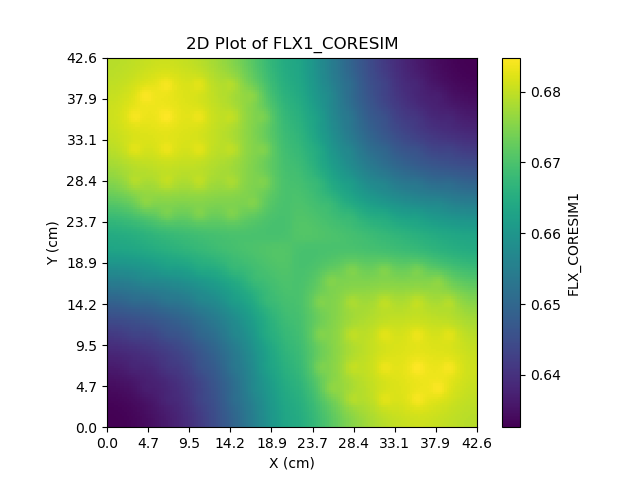
\includegraphics[width=\linewidth]{figures/OBJECTIVES1_TEST02_2DMG_C3_VandV_ADJOINT_FLX_CORESIM_G1.png}
        \end{subfigure}
        \hfill
        \begin{subfigure}{.48\textwidth}
          \centering
          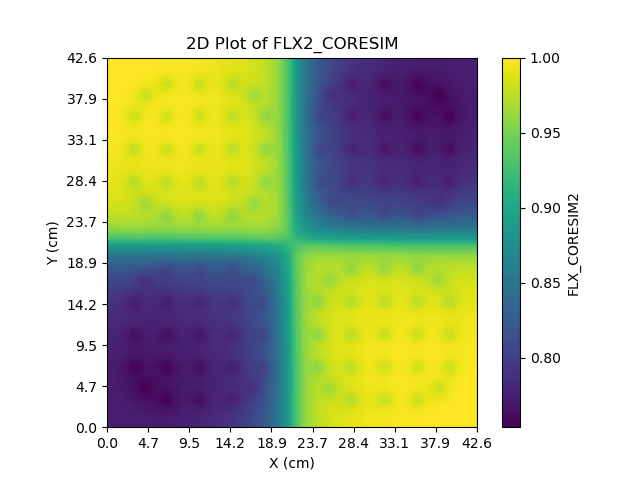
\includegraphics[width=\linewidth]{figures/OBJECTIVES1_TEST02_2DMG_C3_VandV_ADJOINT_FLX_CORESIM_G2.png}
        \end{subfigure}
        \caption{Adjoint flux results from CORE SIM+}
        \label{fig:C3_adj_results_flx}
\end{figure}
\begin{figure}[H]
        \centering
        \begin{subfigure}{.48\textwidth}
          \centering
          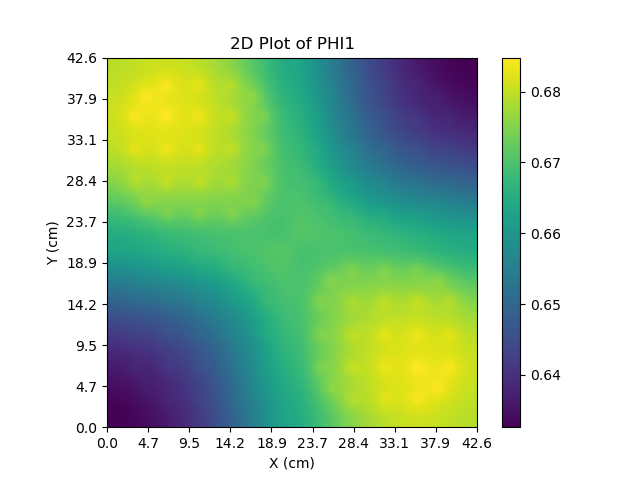
\includegraphics[width=\linewidth]{figures/OBJECTIVES1_TEST02_2DMG_C3_VandV_ADJOINT_PHI_G1.png}
        \end{subfigure}
        \hfill
        \begin{subfigure}{.48\textwidth}
          \centering
          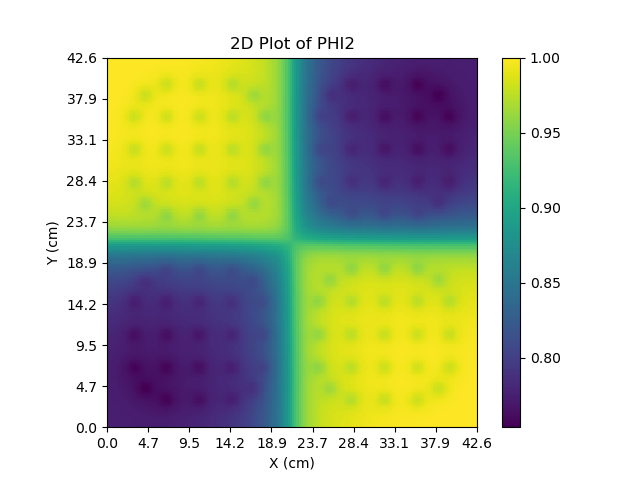
\includegraphics[width=\linewidth]{figures/OBJECTIVES1_TEST02_2DMG_C3_VandV_ADJOINT_PHI_G2.png}
        \end{subfigure}
        \caption{Adjoint flux results from the developed solver}
        \label{fig:C3_adj_results_phi}
\end{figure}
\begin{figure}[H]
        \centering
        \begin{subfigure}{.48\textwidth}
          \centering
          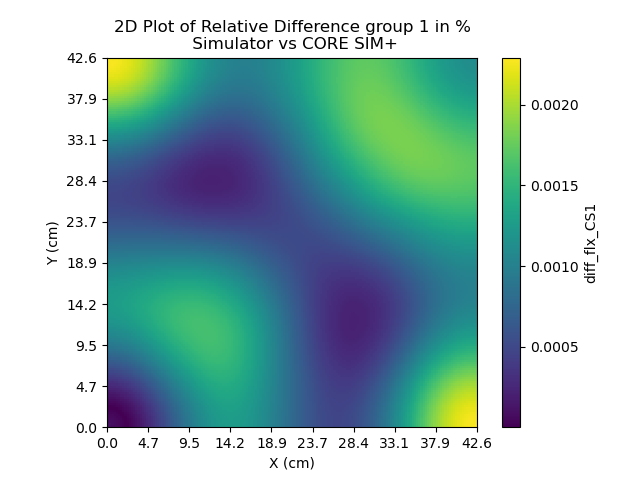
\includegraphics[width=\linewidth]{figures/OBJECTIVES1_TEST02_2DMG_C3_VandV_ADJOINT_diff_flx_CS_G1.png}
        \end{subfigure}
        \hfill
        \begin{subfigure}{.48\textwidth}
          \centering
          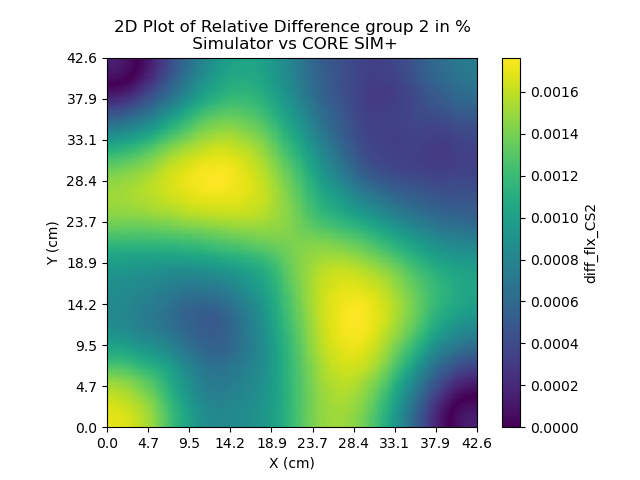
\includegraphics[width=\linewidth]{figures/OBJECTIVES1_TEST02_2DMG_C3_VandV_ADJOINT_diff_flx_CS_G2.png}
        \end{subfigure}
        \caption{Difference of adjoint flux between CORE SIM+ and the solver}
        \label{fig:C3_adj_results_diff_phi}
\end{figure}

As seen in Figure \ref{fig:C3_adj_results_flx}, Figure \ref{fig:C3_adj_results_phi}, and Figure \ref{fig:C3_adj_results_diff_phi}, the results show that the solver agrees well with CORE SIM+. Similar to the forward case, the error is less than 1\% for the adjoint flux. This shows that the solver works well for 2D rectangular geometries to calculate adjoint equation.

\subsection{Neutron Noise Solution}

The neutron noise solutions from CORE SIM+, the developed solver, and comparison between the simulators are shown in Figures \ref{fig:C3_noise_results_flx} - \ref{fig:C3_noise_results_diff_phi}.
\newpage
\begin{figure}[H]
        \centering
        \begin{subfigure}{.48\textwidth}
          \centering
          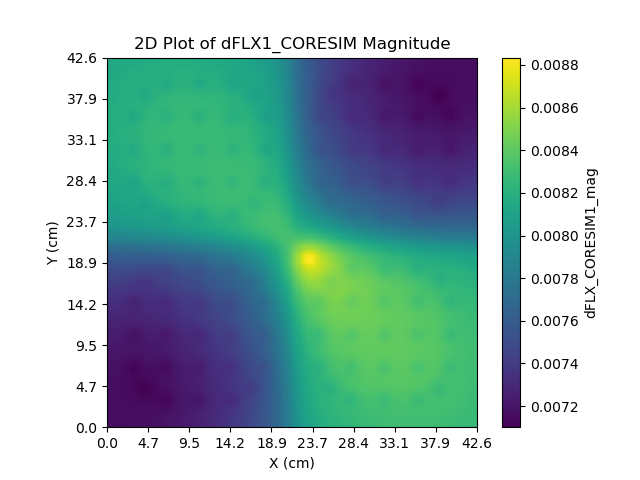
\includegraphics[width=\linewidth]{figures/OBJECTIVES1_TEST02_2DMG_C3_VandV_NOISE_dFLX_CORESIM_magnitude_G1.png}
        \end{subfigure}
        \hfill
        \begin{subfigure}{.48\textwidth}
          \centering
          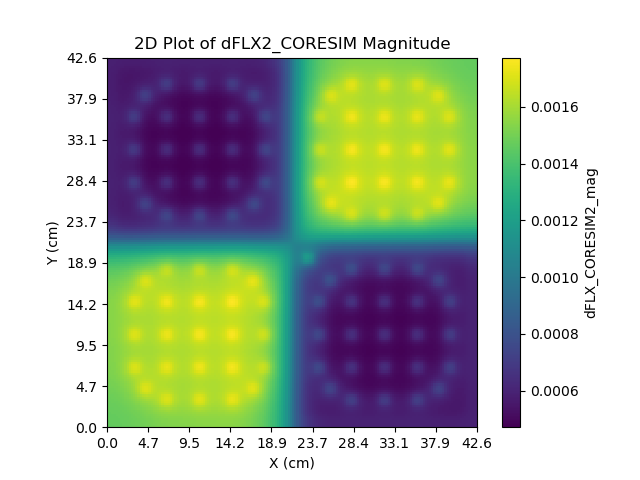
\includegraphics[width=\linewidth]{figures/OBJECTIVES1_TEST02_2DMG_C3_VandV_NOISE_dFLX_CORESIM_magnitude_G2.png}
        \end{subfigure}
\end{figure}
\begin{figure}[H]\ContinuedFloat
        \centering
        \begin{subfigure}{.48\textwidth}
          \centering
          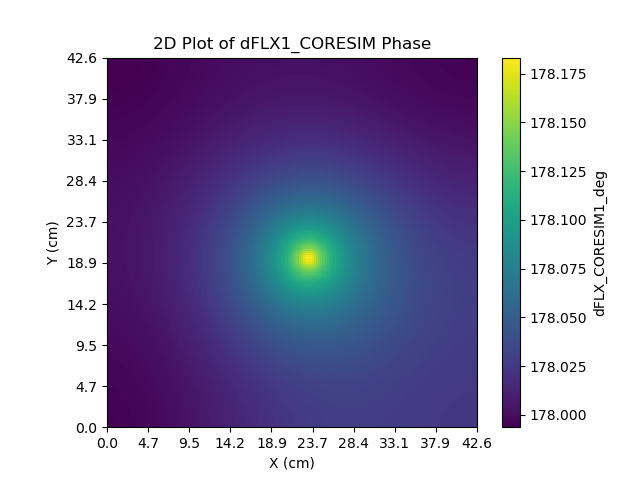
\includegraphics[width=\linewidth]{figures/OBJECTIVES1_TEST02_2DMG_C3_VandV_NOISE_dFLX_CORESIM_phase_G1.png}
        \end{subfigure}
        \hfill
        \begin{subfigure}{.48\textwidth}
          \centering
          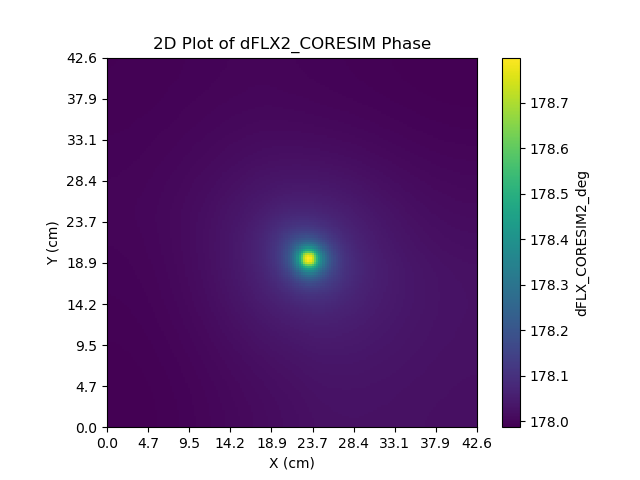
\includegraphics[width=\linewidth]{figures/OBJECTIVES1_TEST02_2DMG_C3_VandV_NOISE_dFLX_CORESIM_phase_G2.png}
        \end{subfigure}
        \caption{Neutron noise results from CORE SIM+}
        \label{fig:C3_noise_results_flx}
\end{figure}

\newpage
\begin{figure}[H]
        \centering
        \begin{subfigure}{.48\textwidth}
          \centering
          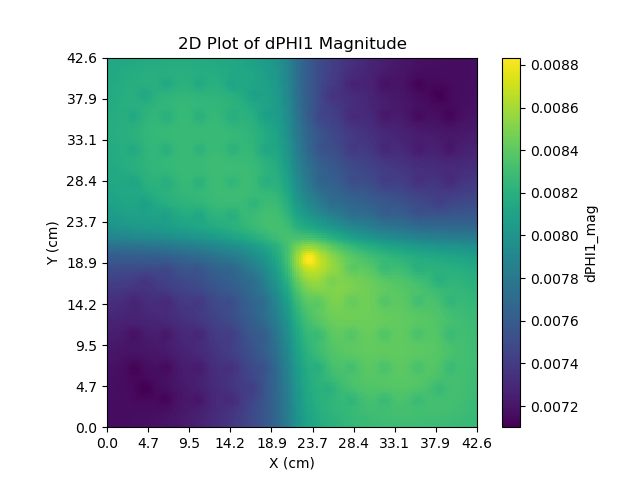
\includegraphics[width=\linewidth]{figures/OBJECTIVES1_TEST02_2DMG_C3_VandV_NOISE_dPHI_magnitude_G1.png}
        \end{subfigure}
        \hfill
        \begin{subfigure}{.48\textwidth}
          \centering
          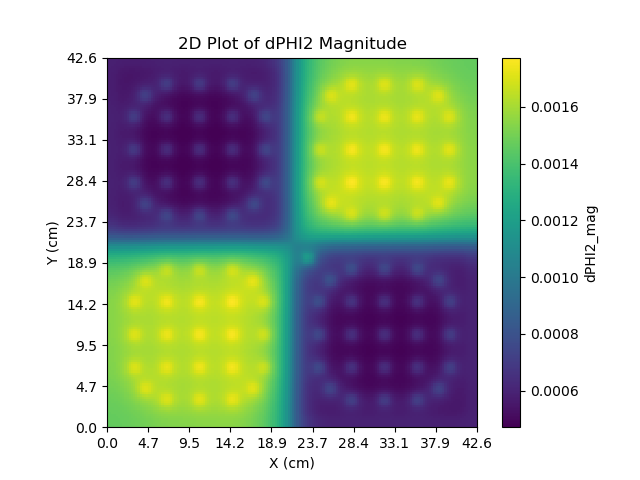
\includegraphics[width=\linewidth]{figures/OBJECTIVES1_TEST02_2DMG_C3_VandV_NOISE_dPHI_magnitude_G2.png}
        \end{subfigure}
\end{figure}
\begin{figure}[H]\ContinuedFloat
        \centering
        \begin{subfigure}{.48\textwidth}
          \centering
          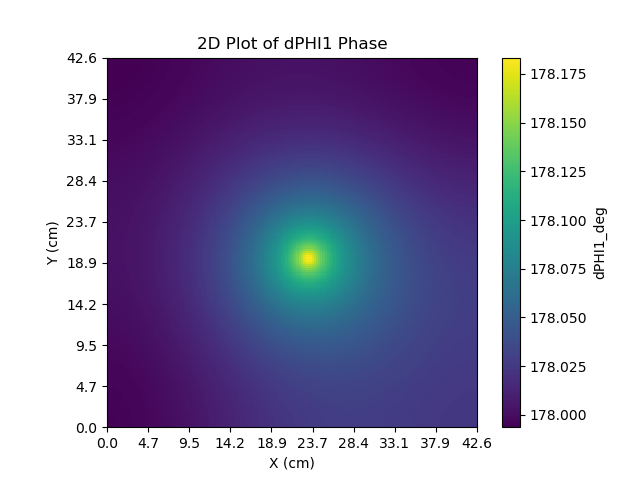
\includegraphics[width=\linewidth]{figures/OBJECTIVES1_TEST02_2DMG_C3_VandV_NOISE_dPHI_phase_G1.png}
        \end{subfigure}
        \hfill
        \begin{subfigure}{.48\textwidth}
          \centering
          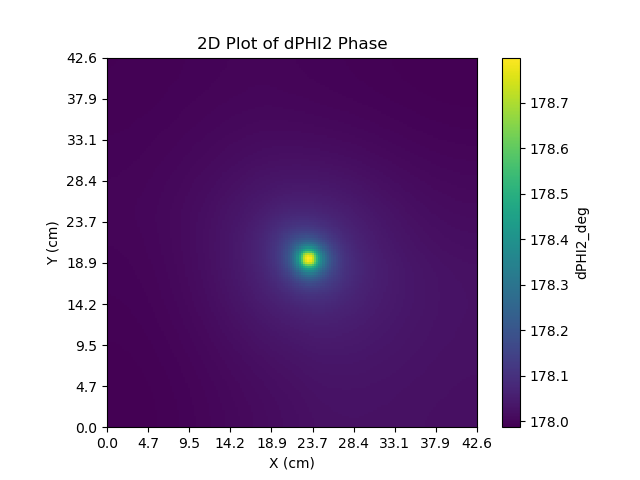
\includegraphics[width=\linewidth]{figures/OBJECTIVES1_TEST02_2DMG_C3_VandV_NOISE_dPHI_phase_G2.png}
        \end{subfigure}
        \caption{Neutron noise results from the developed solver}
        \label{fig:C3_noise_results_phi}
\end{figure}

\newpage
\begin{figure}[H]
        \centering
        \begin{subfigure}{.48\textwidth}
          \centering
          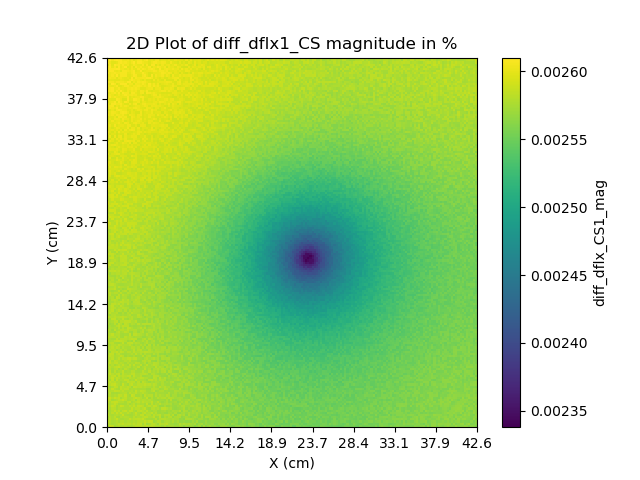
\includegraphics[width=\linewidth]{figures/OBJECTIVES1_TEST02_2DMG_C3_VandV_NOISE_diff_dflx_CS_magnitude_G1.png}
        \end{subfigure}
        \hfill
        \begin{subfigure}{.48\textwidth}
          \centering
          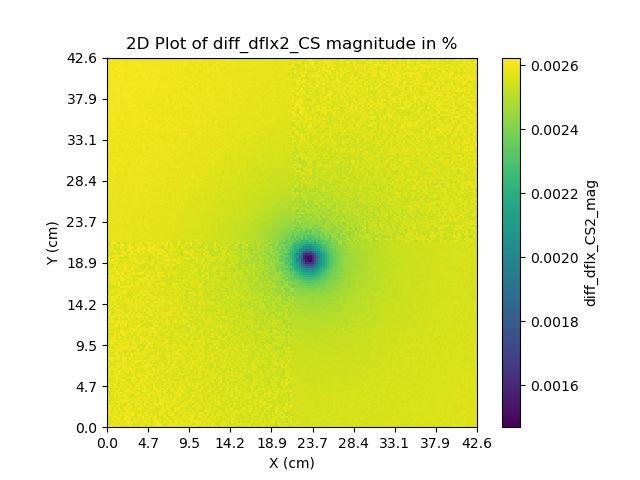
\includegraphics[width=\linewidth]{figures/OBJECTIVES1_TEST02_2DMG_C3_VandV_NOISE_diff_dflx_CS_magnitude_G2.png}
        \end{subfigure}
\end{figure}
\begin{figure}[H]\ContinuedFloat
        \centering
        \begin{subfigure}{.48\textwidth}
          \centering
          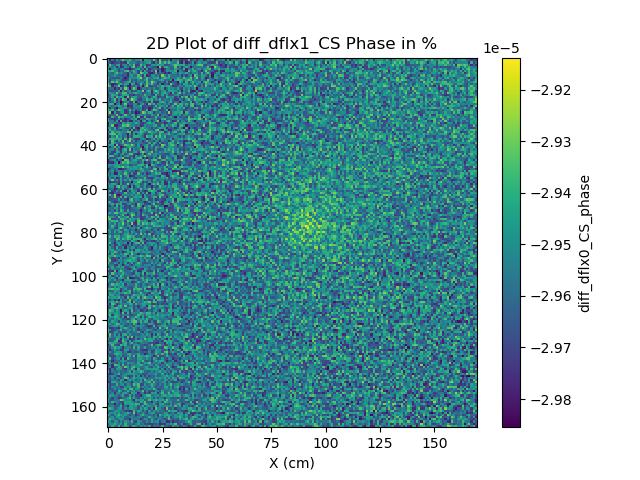
\includegraphics[width=\linewidth]{figures/OBJECTIVES1_TEST02_2DMG_C3_VandV_NOISE_diff_dflx_CS_phase_G1.png}
        \end{subfigure}
        \hfill
        \begin{subfigure}{.48\textwidth}
          \centering
          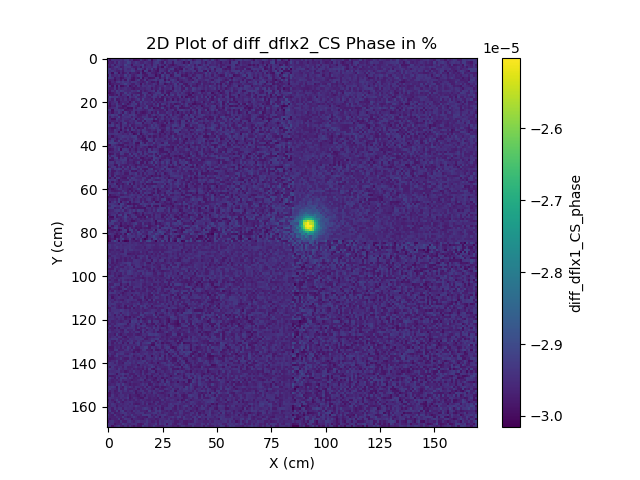
\includegraphics[width=\linewidth]{figures/OBJECTIVES1_TEST02_2DMG_C3_VandV_NOISE_diff_dflx_CS_phase_G2.png}
        \end{subfigure}
        \caption{Difference of neutron noise results between CORE SIM+ and the developed solver}
        \label{fig:C3_noise_results_diff_phi}
\end{figure}

As seen in Figure \ref{fig:C3_noise_results_flx}, Figure \ref{fig:C3_noise_results_phi}, and Figure \ref{fig:C3_noise_results_diff_phi}, the results show that the solutions from the solver agree well with CORE SIM+ solutions. The error is less than 1\% error for the magnitude of the neutron noise, and very low error in the phase of the neutron noise. This shows that the solver works well for 2D rectangular geometries.

\section{3D Westinghouse 4-loop PWR}

In this case, a generic, Western-type PWR is simulated. The overall diameter of the core is 344 cm, and the height of the core is 396.24 cm. This includes the reflector of the core. The active region of the core has a diameter of 322.5 cm and height of 365.76 cm \cite{husseinReactorNeutronNoise2024}. In this case, the simulation includes the reflector regions. It consists of 157 fuel assemblies.

For this case, forward, adjoint, and neutron noise simulations are available in CORE SIM+. These results will be used for comparison. In this dissertation, the forward flux and adjoint flux at the half-plane of the core is compared and reported. For the neutron noise simulation, the plane at which the perturbation happens is reported. The detailed results of the 3D PWR are available in the GitHub repository. The differences between the solver and CORE SIM+ simulation is reported as a relative error defined in Eq. \ref{eq:error1}.

\subsection{Forward Flux Solution}

The forward flux solutions from CORE SIM+, solver, and comparison between the simulators at half-plane ($Z = 27$) are as follows:

\begin{table}[H]
        \centering
        \caption{Eigenvalue comparison of 3D Generic PWR}
        \label{table:PWR3D_fw_results}
        \begin{tabular}{ | M{3.5cm} | M{2cm} | } 
         \hline
         $k_{\text{eff}}$ CORE SIM+ & 1.000965  \\
         \hline
         $k_{\text{eff}}$ solver & 1.000966  \\
         \hline
         Absolute Error (pcm) & 1.0  \\
         \hline
        \end{tabular}
\end{table}

\begin{figure}[H]
        \centering
        \begin{subfigure}{.48\textwidth}
          \centering
          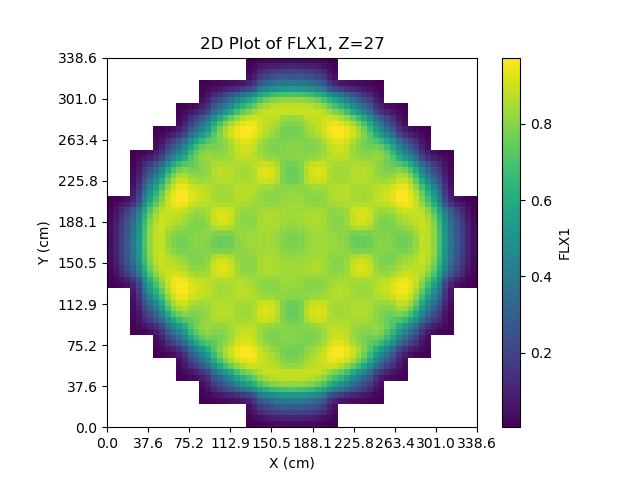
\includegraphics[width=\linewidth]{figures/OBJECTIVES1_TEST06_3DMG_CSTest09_VandV_new_FORWARD_FLX_magnitude_G1_Z27.png}
        \end{subfigure}
        \hfill
        \begin{subfigure}{.48\textwidth}
          \centering
          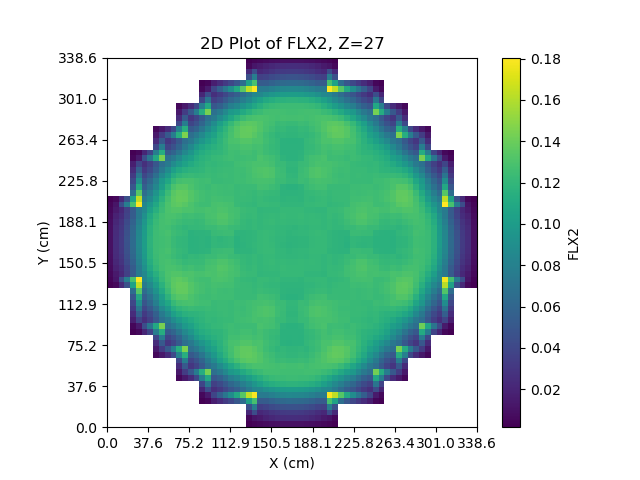
\includegraphics[width=\linewidth]{figures/OBJECTIVES1_TEST06_3DMG_CSTest09_VandV_new_FORWARD_FLX_magnitude_G2_Z27.png}
        \end{subfigure}
        \caption{Forward flux results from CORE SIM+}
        \label{fig:PWR3D_fw_results_flx}
\end{figure}
\begin{figure}[H]
        \centering
        \begin{subfigure}{.48\textwidth}
          \centering
          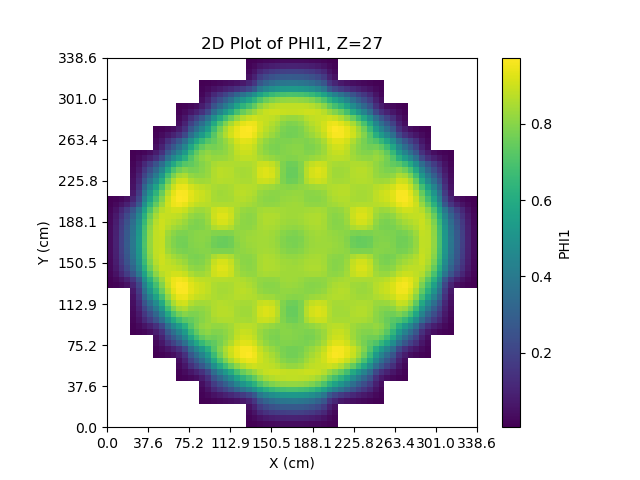
\includegraphics[width=\linewidth]{figures/OBJECTIVES1_TEST06_3DMG_CSTest09_VandV_new_FORWARD_PHI_magnitude_G1_Z27.png}
        \end{subfigure}
        \hfill
        \begin{subfigure}{.48\textwidth}
          \centering
          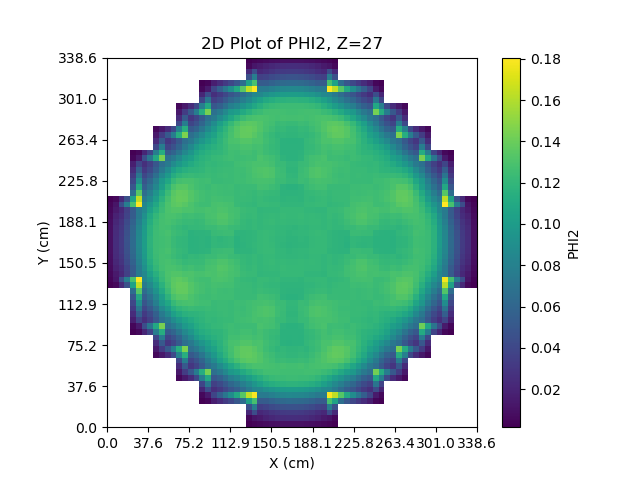
\includegraphics[width=\linewidth]{figures/OBJECTIVES1_TEST06_3DMG_CSTest09_VandV_new_FORWARD_PHI_magnitude_G2_Z27.png}
        \end{subfigure}
        \caption{Forward flux results from the developed solver}
        \label{fig:PWR3D_fw_results_phi}
\end{figure}
\begin{figure}[H]
        \centering
        \begin{subfigure}{.48\textwidth}
          \centering
          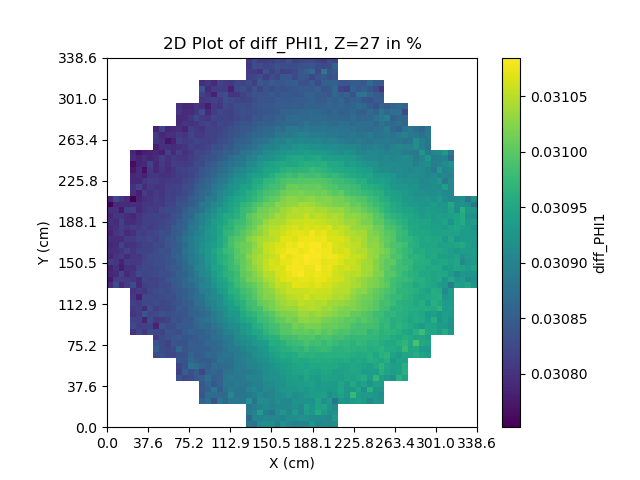
\includegraphics[width=\linewidth]{figures/OBJECTIVES1_TEST06_3DMG_CSTest09_VandV_new_FORWARD_diff_PHI_magnitude_G1_Z27.png}
        \end{subfigure}
        \hfill
        \begin{subfigure}{.48\textwidth}
          \centering
          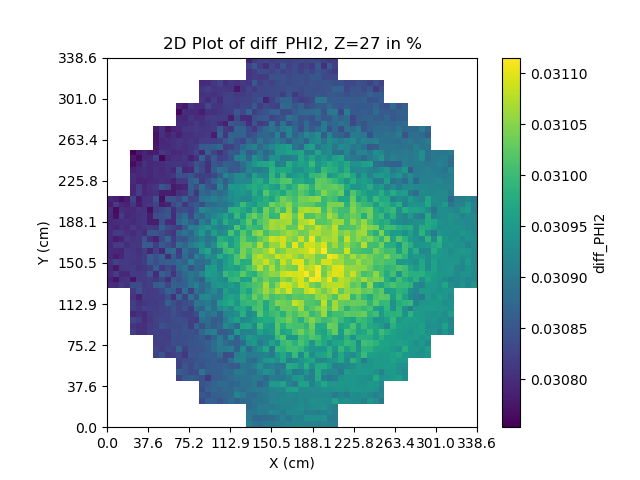
\includegraphics[width=\linewidth]{figures/OBJECTIVES1_TEST06_3DMG_CSTest09_VandV_new_FORWARD_diff_PHI_magnitude_G2_Z27.png}
        \end{subfigure}
        \caption{Difference of forward flux between CORE SIM+ and the solver}
        \label{fig:PWR3D_fw_results_diff_phi}
\end{figure}

The results show that the solver agrees well with CORE SIM+. The $k_{\text{eff}}$ values match between CORE SIM+ and the developed solver with only 1 pcm difference. The error is less than 1\% for the forward flux. This demonstrates that the solver performs effectively for 3D rectangular geometries.

\subsection{Adjoint Flux Solution}

The adjoint flux solutions from CORE SIM+, solver, and comparison between the simulators at half-plane ($Z = 27$) are as follows:

\begin{figure}[H]
        \centering
        \begin{subfigure}{.48\textwidth}
          \centering
          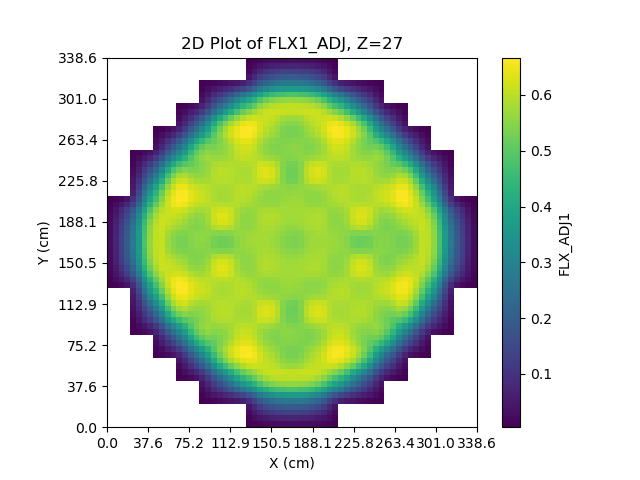
\includegraphics[width=\linewidth]{figures/OBJECTIVES1_TEST06_3DMG_CSTest09_VandV_new_ADJOINT_FLX_ADJ_magnitude_G1_Z27.png}
        \end{subfigure}
        \hfill
        \begin{subfigure}{.48\textwidth}
          \centering
          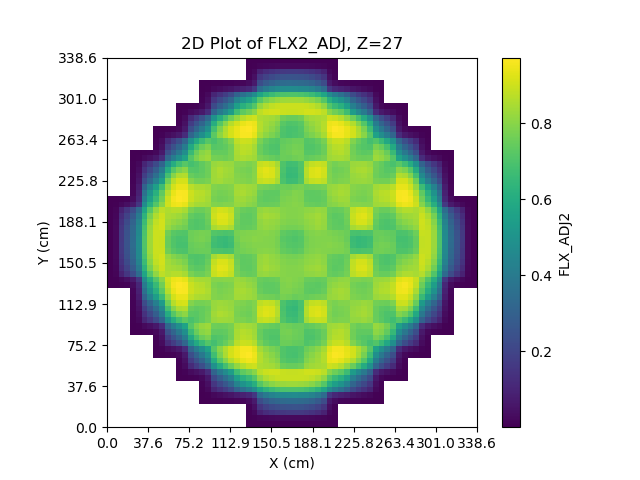
\includegraphics[width=\linewidth]{figures/OBJECTIVES1_TEST06_3DMG_CSTest09_VandV_new_ADJOINT_FLX_ADJ_magnitude_G2_Z27.png}
        \end{subfigure}
        \caption{Adjoint flux results from CORE SIM+}
        \label{fig:PWR3D_adj_results_flx}
\end{figure}
\begin{figure}[H]
        \centering
        \begin{subfigure}{.48\textwidth}
          \centering
          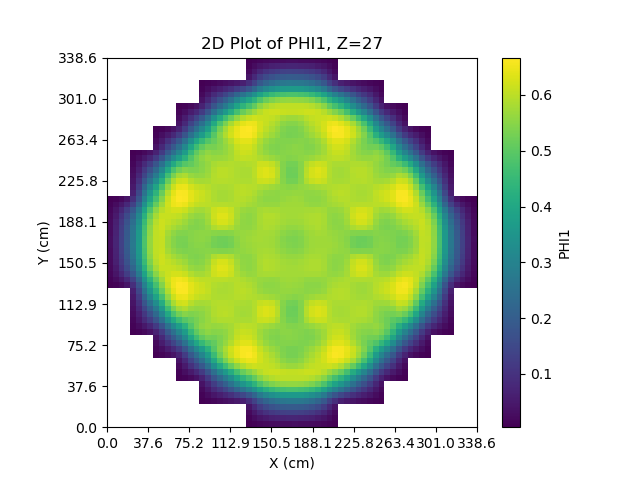
\includegraphics[width=\linewidth]{figures/OBJECTIVES1_TEST06_3DMG_CSTest09_VandV_new_ADJOINT_PHI_magnitude_G1_Z27.png}
        \end{subfigure}
        \hfill
        \begin{subfigure}{.48\textwidth}
          \centering
          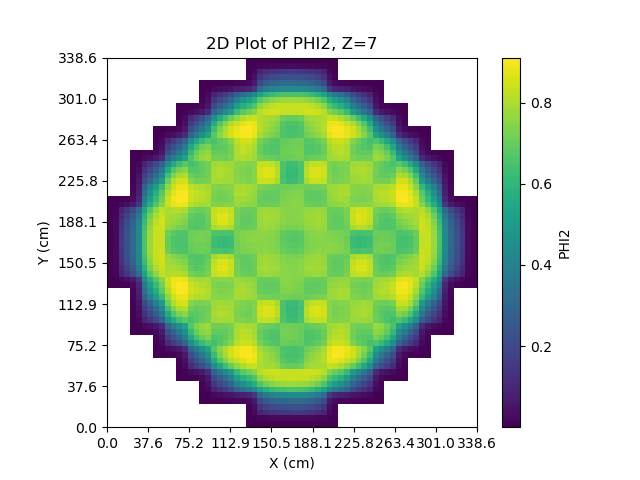
\includegraphics[width=\linewidth]{figures/OBJECTIVES1_TEST06_3DMG_CSTest09_VandV_new_ADJOINT_PHI_magnitude_G2_Z7.png}
        \end{subfigure}
        \caption{Adjoint flux results from the developed solver}
        \label{fig:PWR3D_adj_results_phi}
\end{figure}
\begin{figure}[H]
        \centering
        \begin{subfigure}{.48\textwidth}
          \centering
          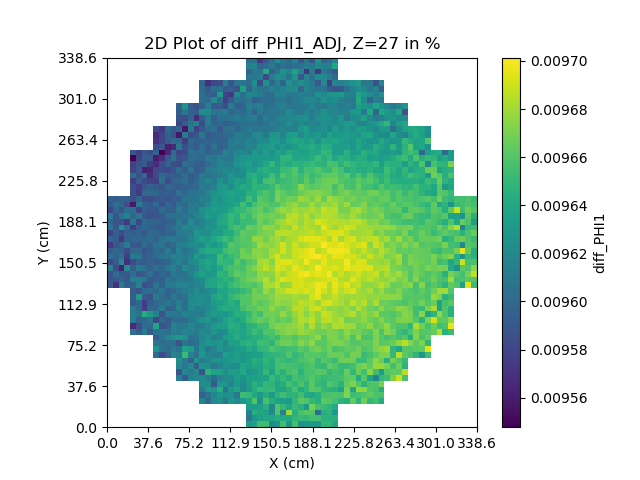
\includegraphics[width=\linewidth]{figures/OBJECTIVES1_TEST06_3DMG_CSTest09_VandV_new_ADJOINT_diff_PHI_magnitude_G1_Z27.png}
        \end{subfigure}
        \hfill
        \begin{subfigure}{.48\textwidth}
          \centering
          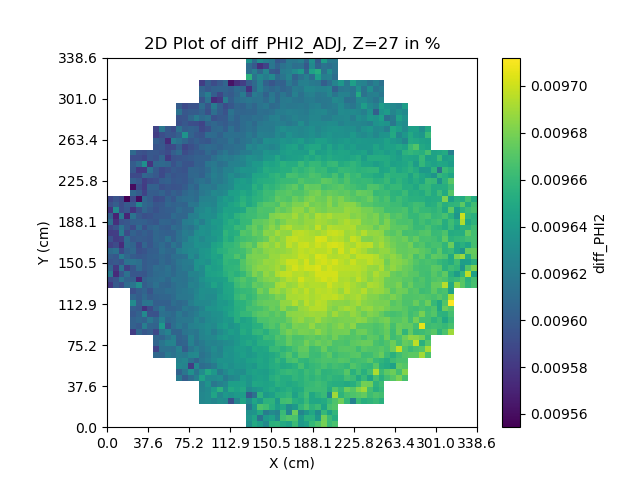
\includegraphics[width=\linewidth]{figures/OBJECTIVES1_TEST06_3DMG_CSTest09_VandV_new_ADJOINT_diff_PHI_magnitude_G2_Z27.png}
        \end{subfigure}
        \caption{Difference of adjoint flux between CORE SIM+ and the solver}
        \label{fig:PWR3D_adj_results_diff_phi}
\end{figure}

The results show that the solver agrees well with CORE SIM+. The error is less than 1\% for the adjoint flux. This indicates that the solver works well for 3D rectangular geometries.

\subsection{Neutron Noise Solution}

In this case, the noise source is defined as a point source at $Z = 10$. Specifically, the noise source is defined as follows:
\begin{equation}
    \delta \Sigma_{t,2}(12, 25, 10, \omega) = 0.05 \Sigma_{t,2} (12, 25, 10)
\end{equation}

This means that the noise source is defined as 5\% perturbation of the thermal total cross sections from their steady state value. The value (12,25,10) indicates the ($x,y,z$) component of the noise source. The neutron noise solutions from CORE SIM+, the developed solver, and the comparison between them at Z=10 are as follows:

\begin{figure}[H]
        \centering
        \begin{subfigure}{.48\textwidth}
          \centering
          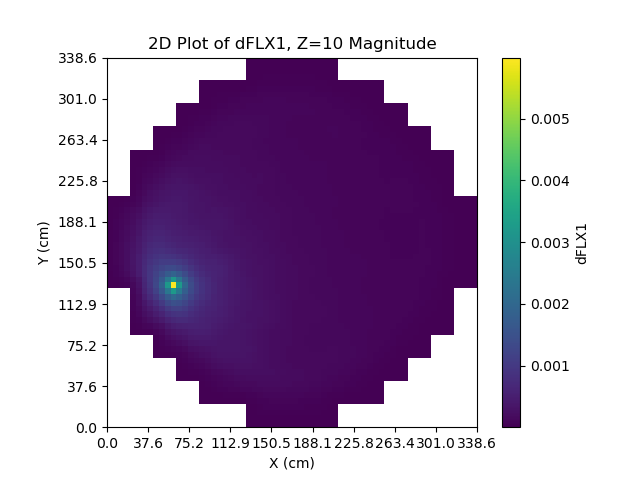
\includegraphics[width=\linewidth]{figures/OBJECTIVES1_TEST06_3DMG_CSTest09_VandV_new_NOISE_dFLX_magnitude_G1_Z10.png}
        \end{subfigure}
        \hfill
        \begin{subfigure}{.48\textwidth}
          \centering
          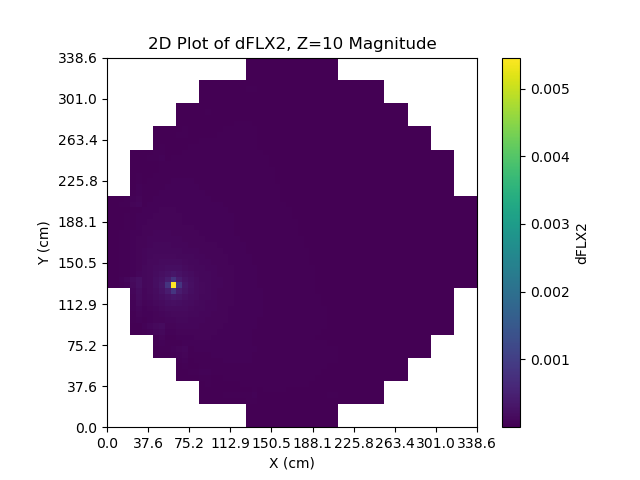
\includegraphics[width=\linewidth]{figures/OBJECTIVES1_TEST06_3DMG_CSTest09_VandV_new_NOISE_dFLX_magnitude_G2_Z10.png}
        \end{subfigure}
\end{figure}
\begin{figure}[H]\ContinuedFloat
        \centering
        \begin{subfigure}{.48\textwidth}
          \centering
          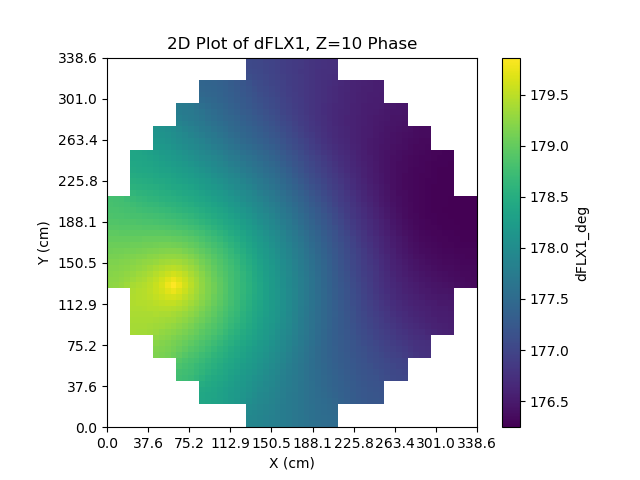
\includegraphics[width=\linewidth]{figures/OBJECTIVES1_TEST06_3DMG_CSTest09_VandV_new_NOISE_dFLX_phase_G1_Z10.png}
        \end{subfigure}
        \hfill
        \begin{subfigure}{.48\textwidth}
          \centering
          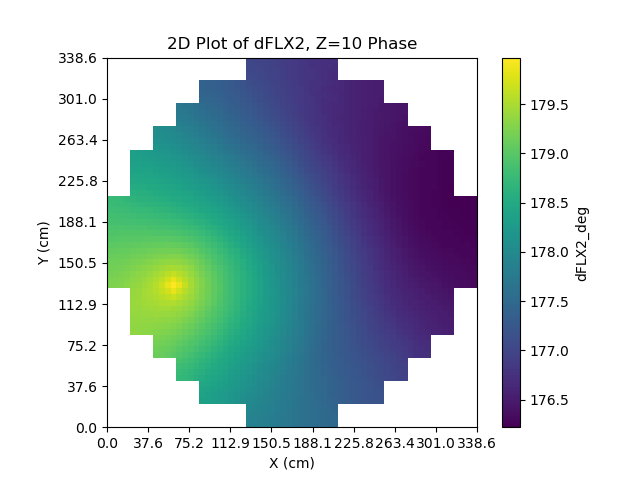
\includegraphics[width=\linewidth]{figures/OBJECTIVES1_TEST06_3DMG_CSTest09_VandV_new_NOISE_dFLX_phase_G2_Z10.png}
        \end{subfigure}
        \caption{Neutron noise results from CORE SIM+}
        \label{fig:PWR3D_noise_results_flx}
\end{figure}

\newpage
\begin{figure}[H]
        \centering
        \begin{subfigure}{.48\textwidth}
          \centering
          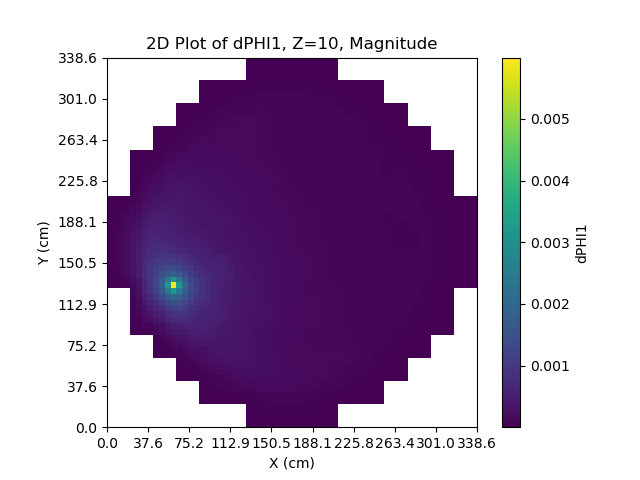
\includegraphics[width=\linewidth]{figures/OBJECTIVES1_TEST06_3DMG_CSTest09_VandV_new_NOISE_dPHI_magnitude_G1_Z10.png}
        \end{subfigure}
        \hfill
        \begin{subfigure}{.48\textwidth}
          \centering
          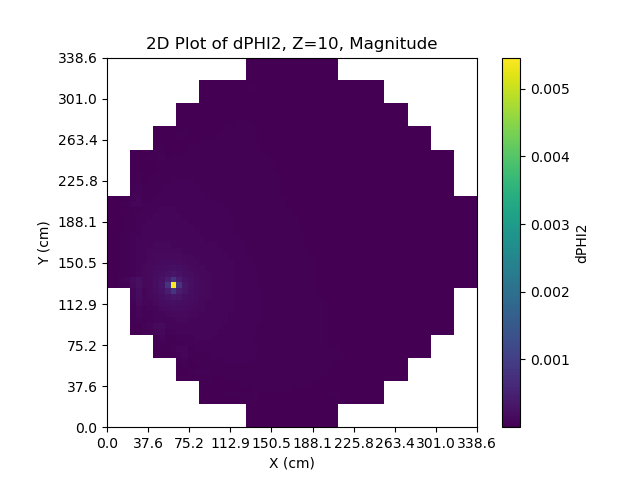
\includegraphics[width=\linewidth]{figures/OBJECTIVES1_TEST06_3DMG_CSTest09_VandV_new_NOISE_dPHI_magnitude_G2_Z10.png}
        \end{subfigure}
\end{figure}
\begin{figure}[H]\ContinuedFloat
        \centering
        \begin{subfigure}{.48\textwidth}
          \centering
          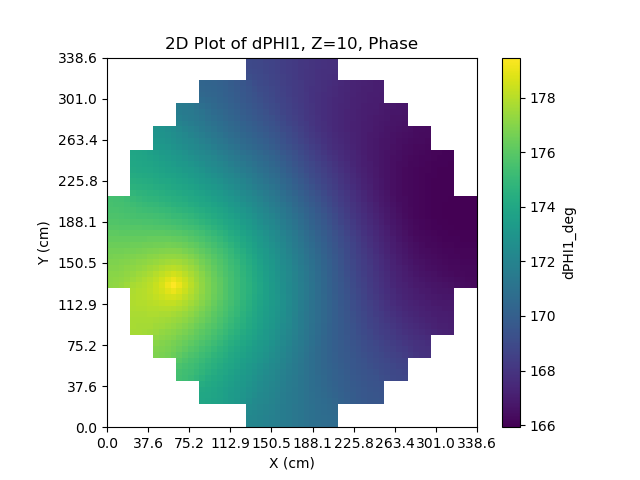
\includegraphics[width=\linewidth]{figures/OBJECTIVES1_TEST06_3DMG_CSTest09_VandV_new_NOISE_dPHI_phase_G1_Z10.png}
        \end{subfigure}
        \hfill
        \begin{subfigure}{.48\textwidth}
          \centering
          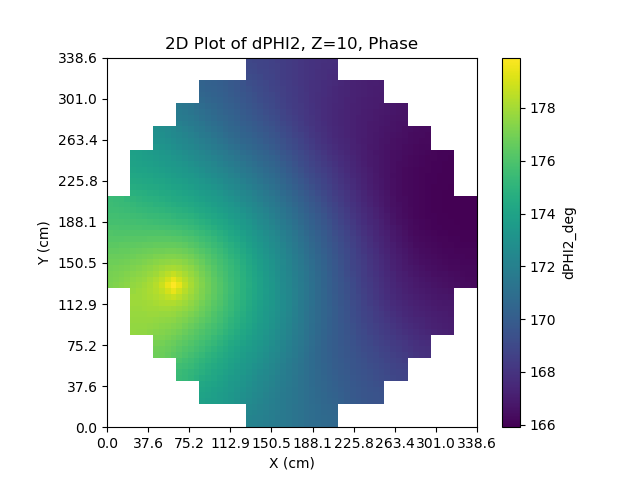
\includegraphics[width=\linewidth]{figures/OBJECTIVES1_TEST06_3DMG_CSTest09_VandV_new_NOISE_dPHI_phase_G2_Z10.png}
        \end{subfigure}
        \caption{Neutron noise results from the developed solver}
        \label{fig:PWR3D_noise_results_phi}
\end{figure}

\newpage
\begin{figure}[H]
        \centering
        \begin{subfigure}{.48\textwidth}
          \centering
          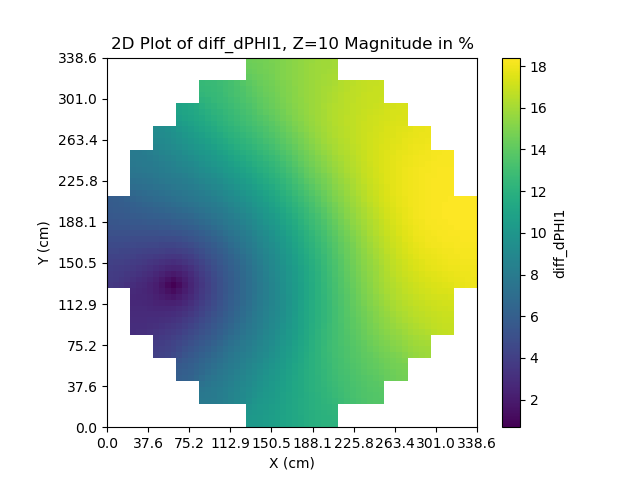
\includegraphics[width=\linewidth]{figures/OBJECTIVES1_TEST06_3DMG_CSTest09_VandV_new_NOISE_diff_dPHI_magnitude_G1_Z10.png}
        \end{subfigure}
        \hfill
        \begin{subfigure}{.48\textwidth}
          \centering
          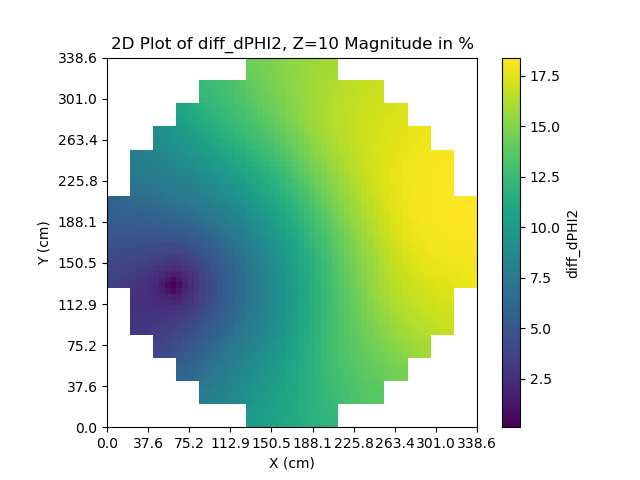
\includegraphics[width=\linewidth]{figures/OBJECTIVES1_TEST06_3DMG_CSTest09_VandV_new_NOISE_diff_dPHI_magnitude_G2_Z10.png}
        \end{subfigure}
\end{figure}
\begin{figure}[H]\ContinuedFloat
        \centering
        \begin{subfigure}{.48\textwidth}
          \centering
          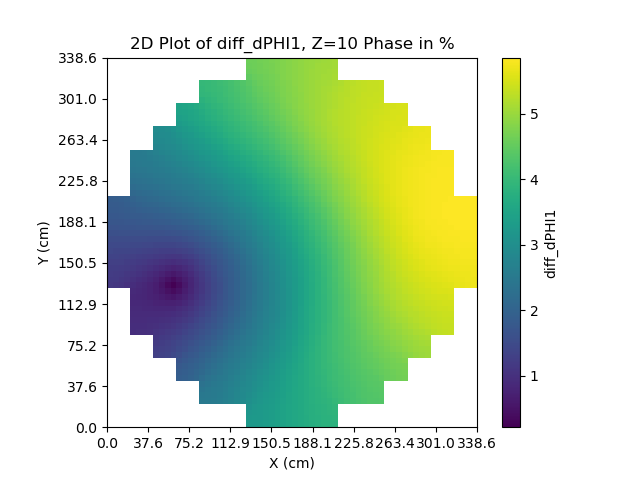
\includegraphics[width=\linewidth]{figures/OBJECTIVES1_TEST06_3DMG_CSTest09_VandV_new_NOISE_diff_dPHI_phase_G1_Z10.png}
        \end{subfigure}
        \hfill
        \begin{subfigure}{.48\textwidth}
          \centering
          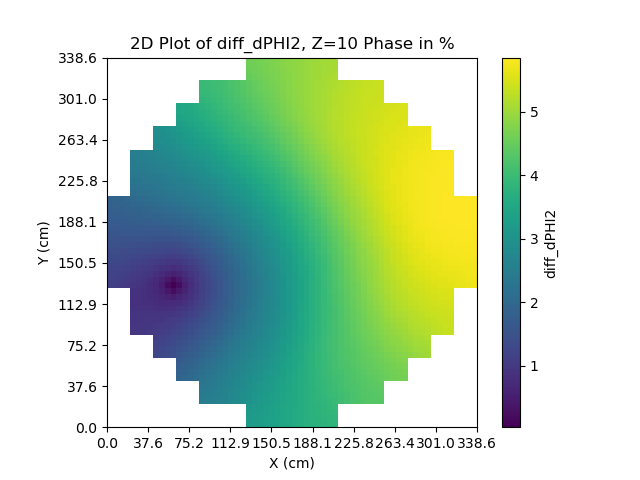
\includegraphics[width=\linewidth]{figures/OBJECTIVES1_TEST06_3DMG_CSTest09_VandV_new_NOISE_diff_dPHI_phase_G2_Z10.png}
        \end{subfigure}
        \caption{Difference of neutron noise results between CORE SIM+ and the developed solver}
        \label{fig:PWR3D_noise_results_diff_phi}
\end{figure}

The results show that the solutions generated by the solver agree well with those from CORE SIM+. The error is higher at the periphery for the magnitude of the neutron noise, and a maximum of 5\% for the phase of the neutron noise. The increase of error in the periphery is caused by the fact that the neutron noise in the periphery is close to zero. As a result, even small absolute deviations in the reconstructed flux can lead to disproportionately large relative errors. In general, the overall results show that the solver works well for 3D rectangular geometries.

\section{2D BIBLIS Benchmark}

The 2D BIBLIS Benchmark, referred to the first nuclear power plant build in the municipality of Biblis (Germany), is is a realistic and highly non-separable 2-group problem representative of an actual operating pressurized water reactor (PWR) with a checker-board-loaded core \cite{mullerBenchmarkingMultigroupDiffusion1991}. The homogenized fuel assemblies with widths of 23.1226 cm and seven different compositions are present in the core which is surrounded by a 23.1226 cm homogenized reflector (i.e. the baffle is bomogenized with the water reflector) with vacuum external boundary conditions. The particular configuration used in this work is that corresponding to the "rods out" case for which the cross section data were taken from a paper by \cite{hebertApplicationHermiteMethod1985}. A complete description of this problem is provided in Figure \ref{fig:2DBIBLIS} and Table \ref{table:2DBIBLISXS}. 

\begin{figure}[H]
        \centering
        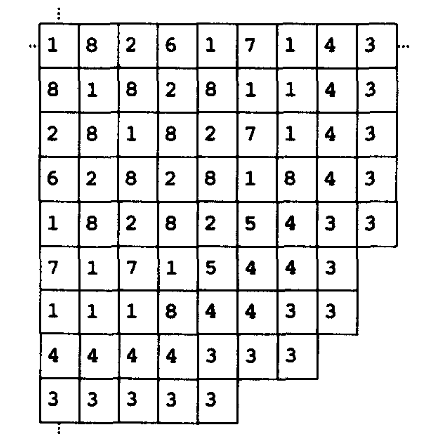
\includegraphics[width=0.45\textwidth]{figures/2DBIBLIS.png}
        \caption{Quarter core configuration of 2D BIBLIS Benchmark (obtained from \cite{mullerBenchmarkingMultigroupDiffusion1991})}
        \label{fig:2DBIBLIS}
\end{figure}

\begin{table}[H]
        \centering
        \caption{Homogenized cross-section data of 2D BIBLIS Benchmark (obtained from \cite{mullerBenchmarkingMultigroupDiffusion1991})}
        \label{table:2DBIBLISXS}
        \begin{tabular}{ | M{1.5cm} | M{1cm} | M{1.5cm} | M{1.5cm} | M{1.5cm} | M{1.5cm} | M{1.5cm} | } 
         \hline
         \textbf{Material} & \textbf{Group} & \textbf{$D_g$} ($cm$) & \textbf{$\Sigma_{a,g}$} ($cm^{-1}$) & \textbf{$\nu \Sigma_{f,g}$}  ($cm^{-1}$) & \textbf{$\Sigma_{f,g}$}  ($cm^{-1}$) & \textbf{$\Sigma_{s,1 \rightarrow}$}  ($cm^{-1}$)\\
         \hline
         \multirow{2}{*}{1} & 1 & 1.4360 & 0.0095042 & 0.0058708 & 0.0023768 & \\
         \cline{2-7}        & 2 & 0.3635 & 0.0750580 & 0.0960670 & 0.0388940 & 0.017754 \\
         \hline
         \multirow{2}{*}{2} & 1 & 1.4366 & 0.0096785 & 0.0061908 & 0.0025064 & \\
         \cline{2-7}        & 2 & 0.3636 & 0.0784360 & 0.1035800 & 0.0419350 & 0.017621 \\
         \hline
         \multirow{2}{*}{3} & 1 & 1.3200 & 0.0026562 & 0.0000000 & 0.0000000 & \\
         \cline{2-7}        & 2 & 0.2772 & 0.0715960 & 0.0000000 & 0.0000000 & 0.023106 \\
         \hline
         \multirow{2}{*}{4} & 1 & 1.4389 & 0.0103630 & 0.0074527 & 0.0030173 & \\
         \cline{2-7}        & 2 & 0.3638 & 0.0914080 & 0.1323600 & 0.0535870 & 0.017101 \\
         \hline
         \multirow{2}{*}{5} & 1 & 1.4381 & 0.0100030 & 0.0061908 & 0.0025064 & \\
         \cline{2-7}        & 2 & 0.3665 & 0.0848280 & 0.1035800 & 0.0419350 & 0.017192 \\
         \hline
         \multirow{2}{*}{6} & 1 & 1.4385 & 0.0101320 & 0.0064285 & 0.0026026 & \\
         \cline{2-7}        & 2 & 0.3665 & 0.0873140 & 0.1091100 & 0.0441740 & 0.017192 \\
         \hline
         \multirow{2}{*}{7} & 1 & 1.4389 & 0.0101650 & 0.0061908 & 0.0025064 & \\
         \cline{2-7}        & 2 & 0.3679 & 0.0880240 & 0.1035800 & 0.0419350 & 0.017125 \\
         \hline
         \multirow{2}{*}{8} & 1 & 1.4393 & 0.0102940 & 0.0064285 & 0.0026026 & \\
         \cline{2-7}        & 2 & 0.3680 & 0.0905100 & 0.1091100 & 0.0441740 & 0.017027 \\
         \hline
        \end{tabular}
\end{table}

The 2D BIBLIS Benchmark has been simulated in FEMFFUSION \cite{vidal-ferrandizFEMFFUSIONFiniteElement2023} and compared with the developed solver. The results are as follows:

\subsection{Forward Simulation}
\begin{table}[H]
        \centering
        \caption{Eigenvalue comparison of 2D BIBLIS Benchmark}
        \label{table:BIBLIS_fw_results}
        \begin{tabular}{ | M{3.5cm} | M{2cm} | } 
         \hline
         $k_{\text{eff}}$ FEMFFUSION & 1.02535  \\
         \hline
         $k_{\text{eff}}$ solver & 1.02519  \\
         \hline
         Absolute Error (pcm) & 16.0  \\
         \hline
        \end{tabular}
\end{table}

\begin{figure}[H]
        \centering
        \begin{subfigure}{.48\textwidth}
          \centering
          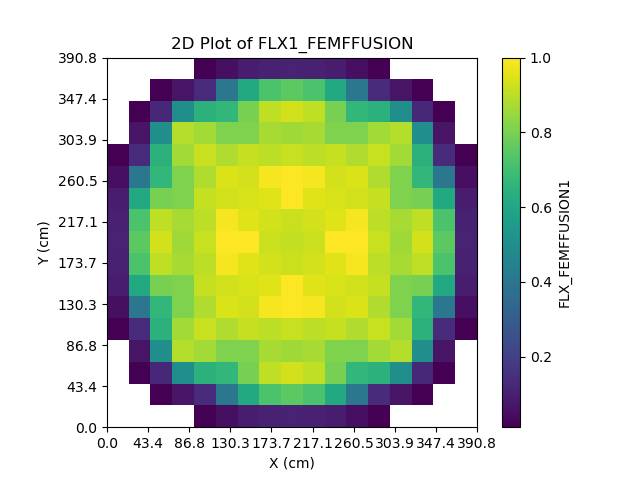
\includegraphics[width=\linewidth]{figures/OBJECTIVES1_TEST03_2DMG_BIBLIS_VandV_FORWARD_FLX_FEMFFUSION_G1.png}
        \end{subfigure}
        \hfill
        \begin{subfigure}{.48\textwidth}
          \centering
          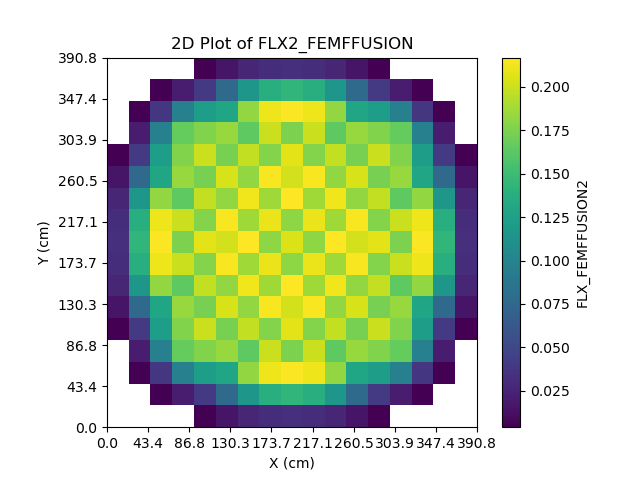
\includegraphics[width=\linewidth]{figures/OBJECTIVES1_TEST03_2DMG_BIBLIS_VandV_FORWARD_FLX_FEMFFUSION_G2.png}
        \end{subfigure}
        \caption{Forward flux results from FEMFFUSION}
        \label{fig:BIBLIS_fw_results_flx}
\end{figure}
\begin{figure}[H]
        \centering
        \begin{subfigure}{.48\textwidth}
          \centering
          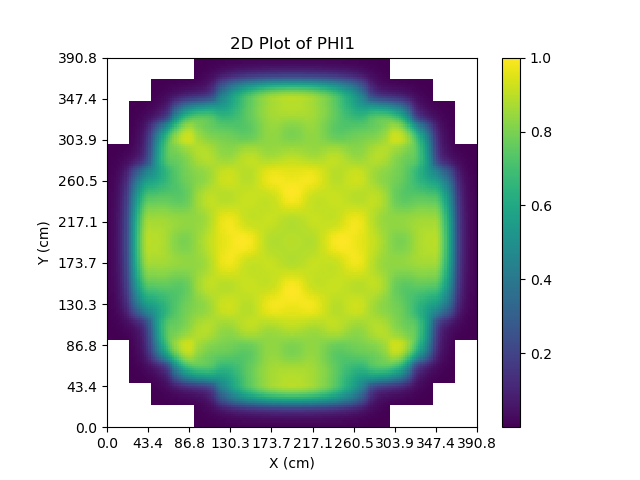
\includegraphics[width=\linewidth]{figures/OBJECTIVES1_TEST03_2DMG_BIBLIS_VandV_FORWARD_PHI_G1.png}
        \end{subfigure}
        \hfill
        \begin{subfigure}{.48\textwidth}
          \centering
          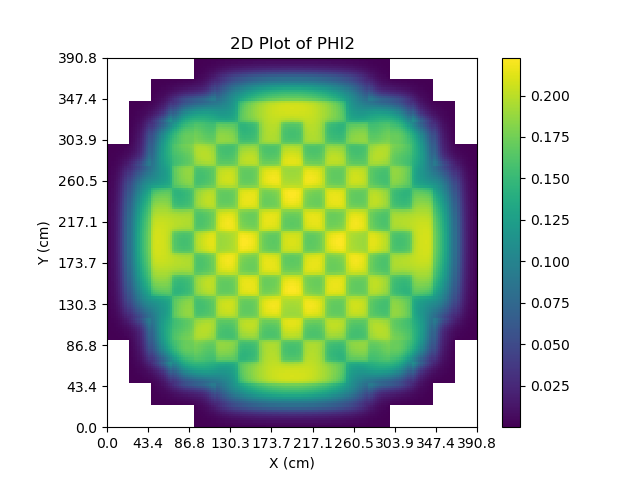
\includegraphics[width=\linewidth]{figures/OBJECTIVES1_TEST03_2DMG_BIBLIS_VandV_FORWARD_PHI_G2.png}
        \end{subfigure}
        \caption{Forward flux results from the developed solver}
        \label{fig:BIBLIS_fw_results_phi}
\end{figure}
\begin{figure}[H]
        \centering
        \begin{subfigure}{.48\textwidth}
          \centering
          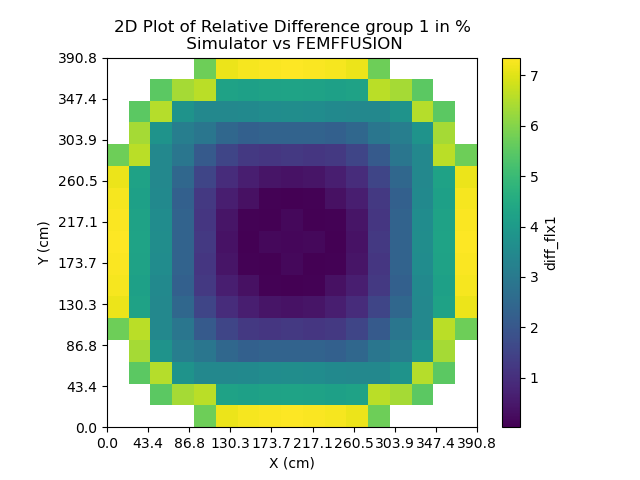
\includegraphics[width=\linewidth]{figures/OBJECTIVES1_TEST03_2DMG_BIBLIS_VandV_FORWARD_diff_flx_G1.png}
        \end{subfigure}
        \hfill
        \begin{subfigure}{.48\textwidth}
          \centering
          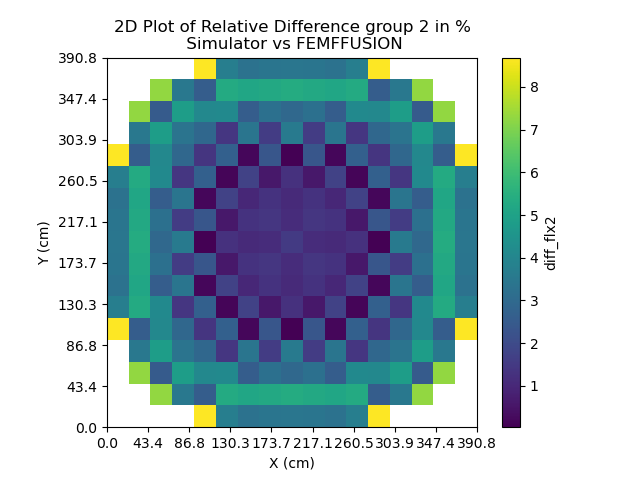
\includegraphics[width=\linewidth]{figures/OBJECTIVES1_TEST03_2DMG_BIBLIS_VandV_FORWARD_diff_flx_G2.png}
        \end{subfigure}
        \caption{Difference of forward flux between FEMFFUSION and the solver}
\end{figure}

The forward results show that some discrepancies are observed between the developed solver and FEMFFUSION. This difference is due to the use of the finite element method in FEMFFUSION, which has different degrees of accuracy compared to the box-scheme finite difference used in the solver. The error in $k_\text{eff}$ is 16 pcm and the maximum error in the neutron flux is about 8\%. Considering this difference in spatial discretization method, the solver generally works well and in a certain degree of agreement with FEMFFUSION.

\subsection{Adjoint Simulation}

\begin{figure}[H]
        \centering
        \begin{subfigure}{.48\textwidth}
          \centering
          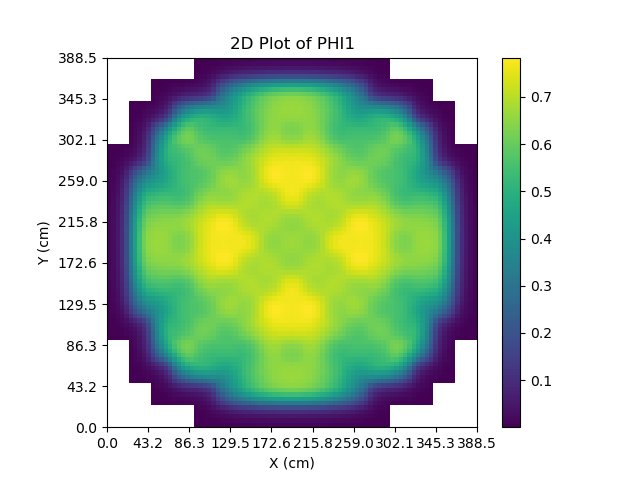
\includegraphics[width=\linewidth]{figures/OBJECTIVES1_TEST03_2DMG_BIBLIS_VandV_ADJOINT_PHI_G1.png}
        \end{subfigure}
        \hfill
        \begin{subfigure}{.48\textwidth}
          \centering
          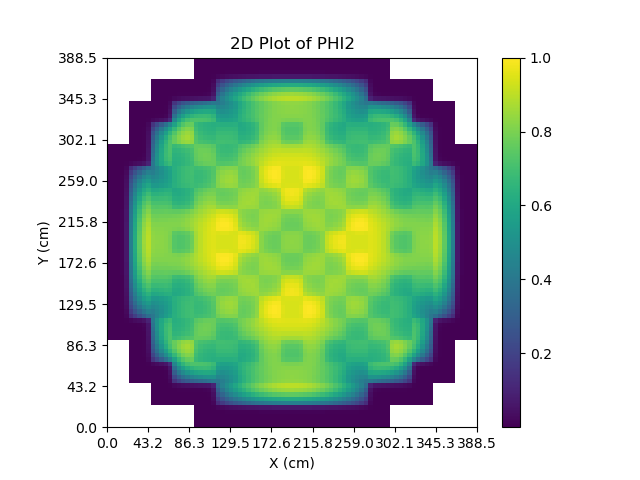
\includegraphics[width=\linewidth]{figures/OBJECTIVES1_TEST03_2DMG_BIBLIS_VandV_ADJOINT_PHI_G2.png}
        \end{subfigure}
        \caption{Adjoint flux results from the developed solver}
        \label{fig:BIBLIS_adj_results_phi}
\end{figure}

There are no direct comparisons available for the adjoint flux solution. However, the results of the adjoint simulation show expected results using the developed solver, with the maximum flux at the thermal group solution. 

\subsection{Neutron Noise Simulation}

For the neutron noise simulation, the noise source is defined as an AVS-type noise source located at the center of the core. The noise sources are defined as follows:
\begin{equation}
    \begin{aligned}
        \delta \Sigma_{a,1} (\textbf{r}_p) &= 0.005 \\
        \delta \Sigma_{a,2} (\textbf{r}_p) &= 0.005 \\
        \delta \Sigma_{s,1\rightarrow2} (\textbf{r}_p) &= 0.005 \\        
    \end{aligned}
\end{equation}

The 2D BIBLIS Benchmark has been simulated in FEMFFUSION \cite{vidal-ferrandizFEMFFUSIONFiniteElement2023} and compared with the developed solver. The results are as follows:

\begin{figure}[H]
        \centering
        \begin{subfigure}{.48\textwidth}
          \centering
          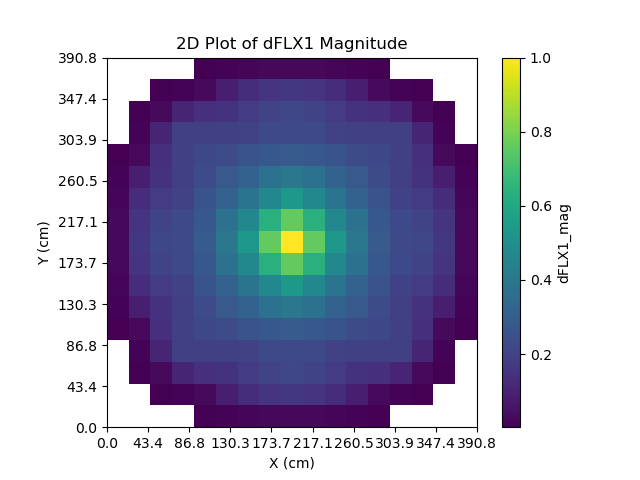
\includegraphics[width=\linewidth]{figures/OBJECTIVES1_TEST03_2DMG_BIBLIS_VandV_NOISE_dFLX_magnitude_G1.png}
        \end{subfigure}
        \hfill
        \begin{subfigure}{.48\textwidth}
          \centering
          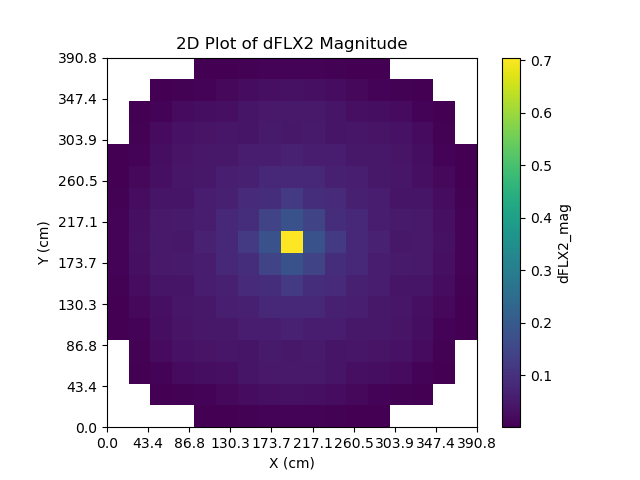
\includegraphics[width=\linewidth]{figures/OBJECTIVES1_TEST03_2DMG_BIBLIS_VandV_NOISE_dFLX_magnitude_G2.png}
        \end{subfigure}
\end{figure}
\begin{figure}[H]\ContinuedFloat
        \centering
        \begin{subfigure}{.48\textwidth}
          \centering
          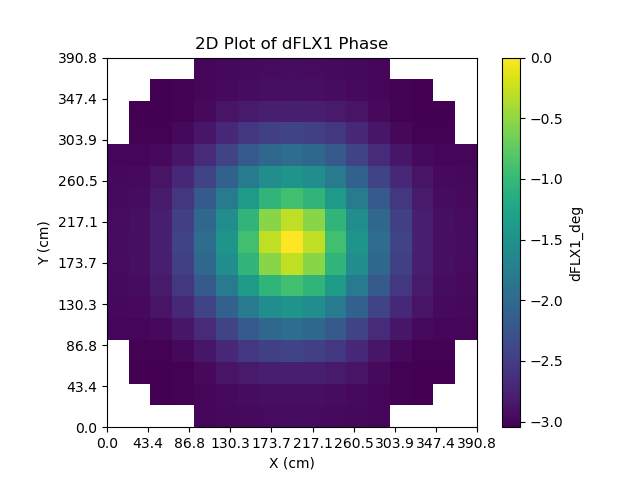
\includegraphics[width=\linewidth]{figures/OBJECTIVES1_TEST03_2DMG_BIBLIS_VandV_NOISE_dFLX_phase_G1.png}
        \end{subfigure}
        \hfill
        \begin{subfigure}{.48\textwidth}
          \centering
          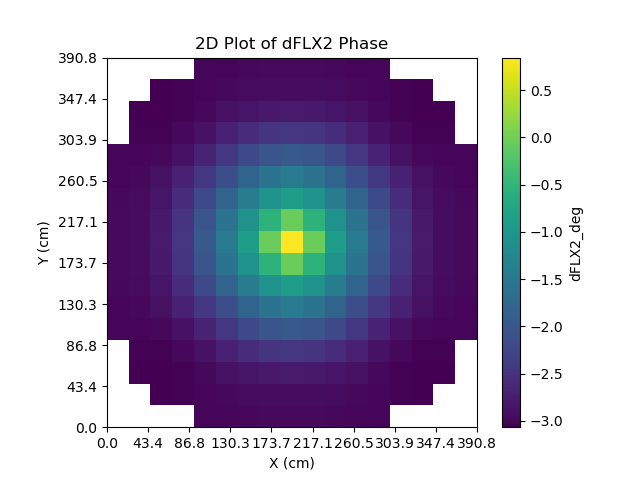
\includegraphics[width=\linewidth]{figures/OBJECTIVES1_TEST03_2DMG_BIBLIS_VandV_NOISE_dFLX_phase_G2.png}
        \end{subfigure}
        \caption{Neutron noise results from FEMFFUSION}
        \label{fig:BIBLIS_noise_results_flx}
\end{figure}

\begin{figure}[H]
        \centering
        \begin{subfigure}{.48\textwidth}
          \centering
          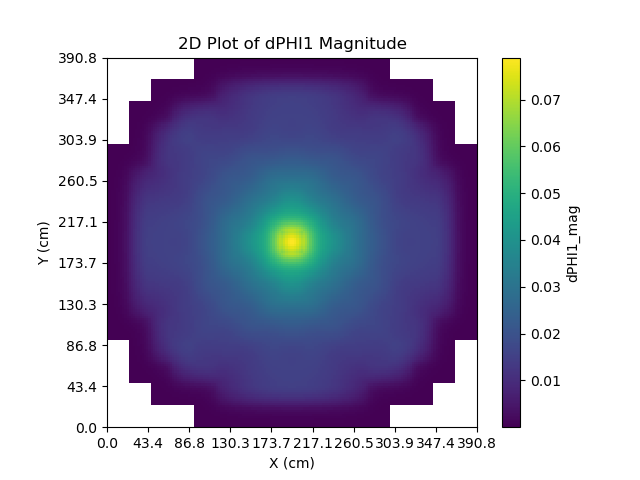
\includegraphics[width=\linewidth]{figures/OBJECTIVES1_TEST03_2DMG_BIBLIS_VandV_NOISE_dPHI_magnitude_G1.png}
        \end{subfigure}
        \hfill
        \begin{subfigure}{.48\textwidth}
          \centering
          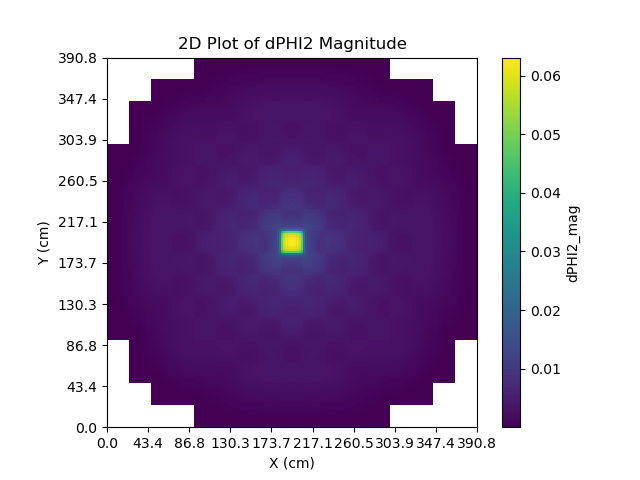
\includegraphics[width=\linewidth]{figures/OBJECTIVES1_TEST03_2DMG_BIBLIS_VandV_NOISE_dPHI_magnitude_G2.png}
        \end{subfigure}
\end{figure}
\begin{figure}[H]\ContinuedFloat
        \centering
        \begin{subfigure}{.48\textwidth}
          \centering
          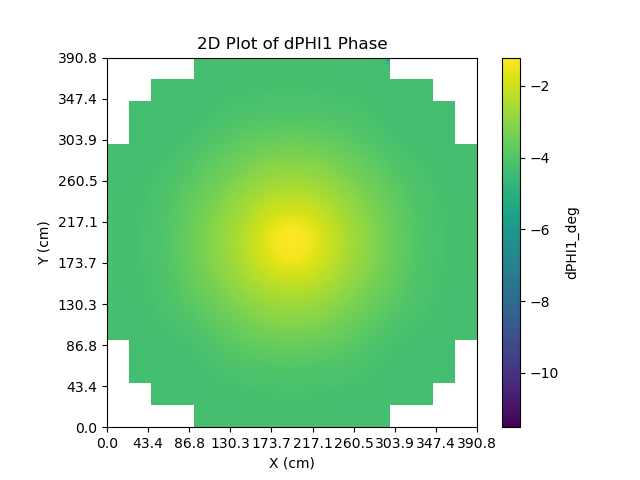
\includegraphics[width=\linewidth]{figures/OBJECTIVES1_TEST03_2DMG_BIBLIS_VandV_NOISE_dPHI_phase_G1.png}
        \end{subfigure}
        \hfill
        \begin{subfigure}{.48\textwidth}
          \centering
          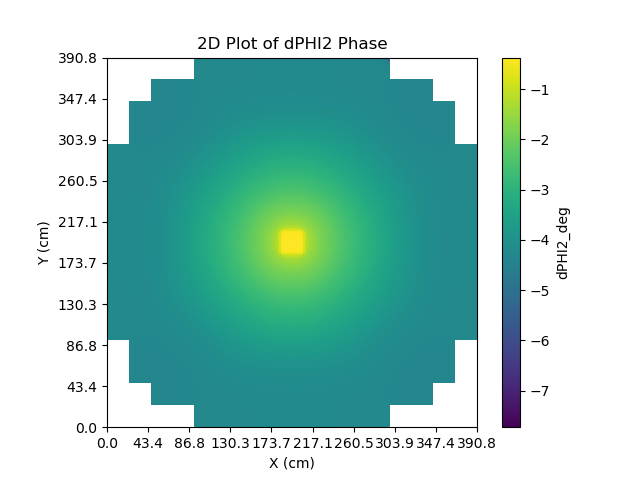
\includegraphics[width=\linewidth]{figures/OBJECTIVES1_TEST03_2DMG_BIBLIS_VandV_NOISE_dPHI_phase_G2.png}
        \end{subfigure}
        \caption{Neutron noise results from the developed solver}
        \label{fig:BIBLIS_noise_results_phi}
\end{figure}

\newpage
\begin{figure}[H]
        \centering
        \begin{subfigure}{.48\textwidth}
          \centering
          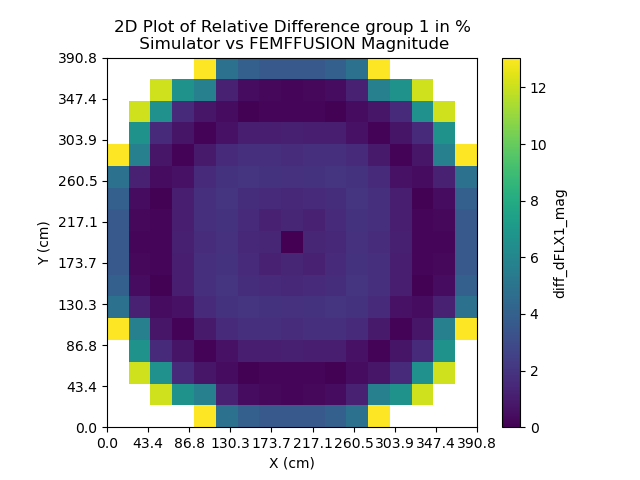
\includegraphics[width=\linewidth]{figures/OBJECTIVES1_TEST03_2DMG_BIBLIS_VandV_NOISE_diff_dFLX_magnitude_G1.png}
        \end{subfigure}
        \hfill
        \begin{subfigure}{.48\textwidth}
          \centering
          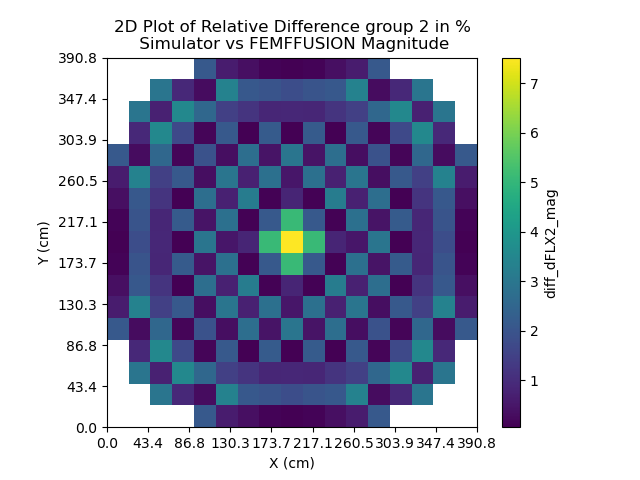
\includegraphics[width=\linewidth]{figures/OBJECTIVES1_TEST03_2DMG_BIBLIS_VandV_NOISE_diff_dFLX_magnitude_G2.png}
        \end{subfigure}
\end{figure}
\begin{figure}[H]\ContinuedFloat
        \centering
        \begin{subfigure}{.48\textwidth}
          \centering
          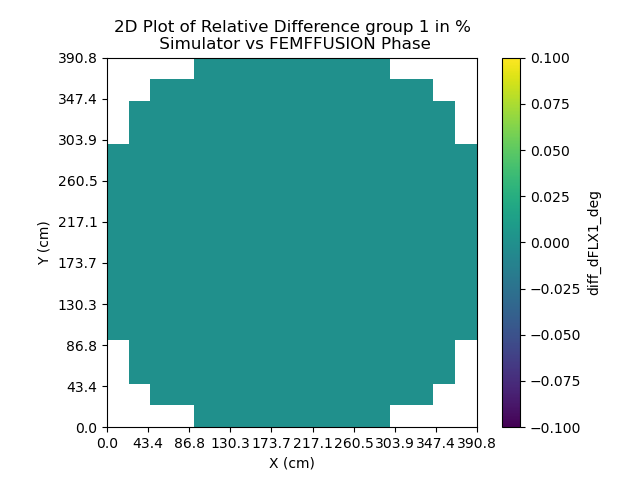
\includegraphics[width=\linewidth]{figures/OBJECTIVES1_TEST03_2DMG_BIBLIS_VandV_NOISE_diff_dFLX_phase_G1.png}
        \end{subfigure}
        \hfill
        \begin{subfigure}{.48\textwidth}
          \centering
          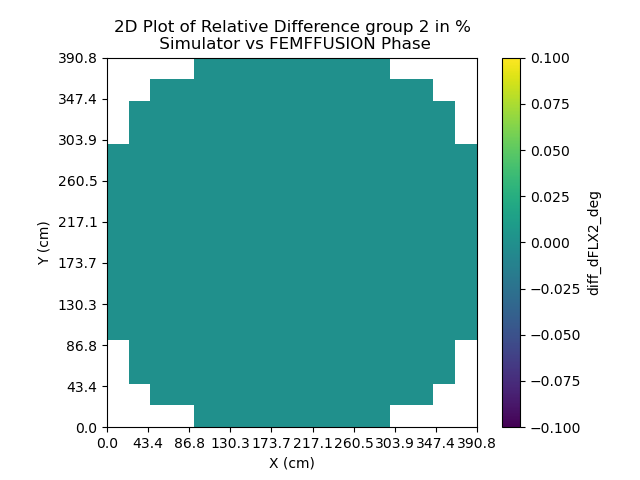
\includegraphics[width=\linewidth]{figures/OBJECTIVES1_TEST03_2DMG_BIBLIS_VandV_NOISE_diff_dFLX_phase_G2.png}
        \end{subfigure}
        \caption{Difference of neutron noise results between FEMFFUSION and the developed solver}
        \label{fig:BIBLIS_noise_results_diff_phi}
\end{figure}

Comparing the results between FEMFFUSION and the developed solver, the results show that the neutron noise solution between FEMFFUSION and the developed solver are in good agreement to each other. The maximum error of the magnitude is about 12\% and it is mainly located at the periphery of the core. Considering this difference in spatial discretization method, the solver generally works well and in a certain degree of agreement with FEMFFUSION.

\section{2D VVER-400}

\subsection{Neutron Noise Solution}

In this case, it is defined that the noise source perturbed the thermal total cross-section.
\begin{equation}
    \delta \Sigma_{t,2}(\textbf{r}_p,\omega) = 0.05 \Sigma_{t,2}(\textbf{r}_p)
\end{equation}
where we define $\textbf{r}_p$ near the center of the core, indicated by yellow hexagon in Figure \ref{fig:2DVVER_source}.
\begin{figure}[H]
        \centering
        \begin{subfigure}{.48\textwidth}
          \centering
          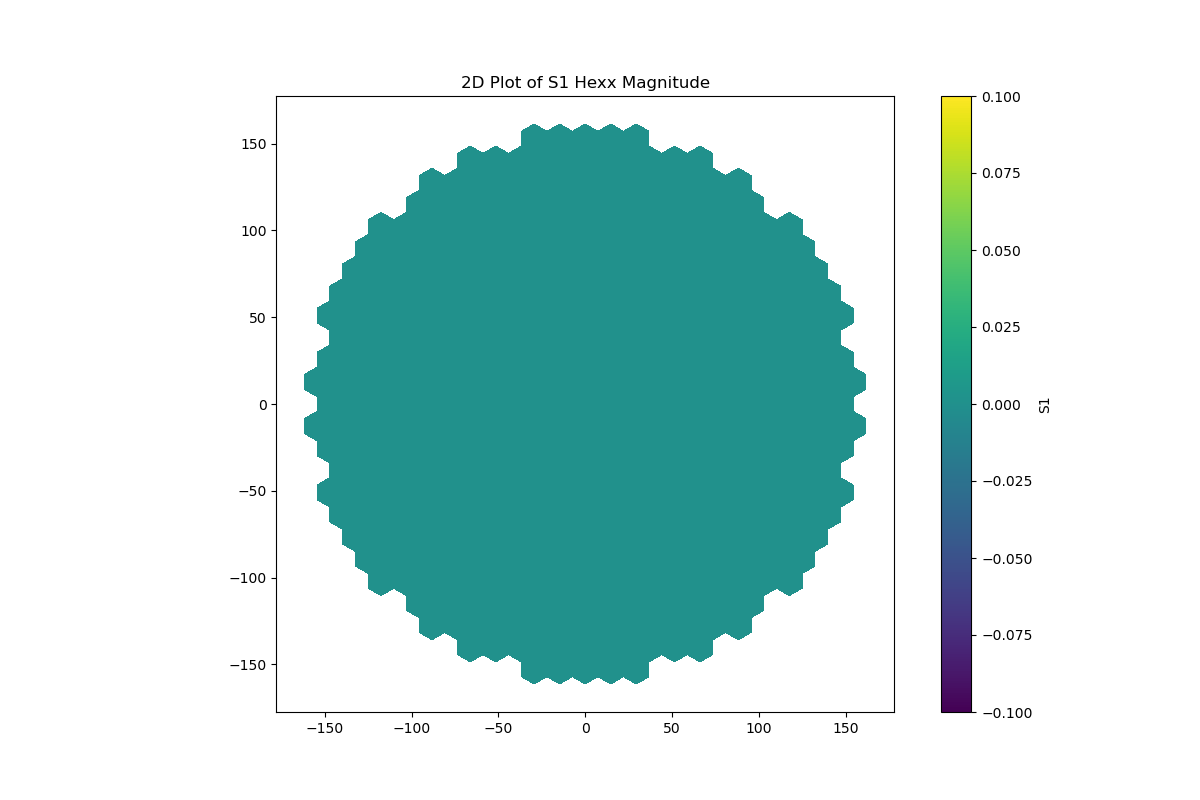
\includegraphics[width=\linewidth]{figures/OBJECTIVES1_TEST05_2DTriMG_VVER400_VandV_level2_NOISE_S_magnitude_G1.png}
        \end{subfigure}
        \hfill
        \begin{subfigure}{.48\textwidth}
          \centering
          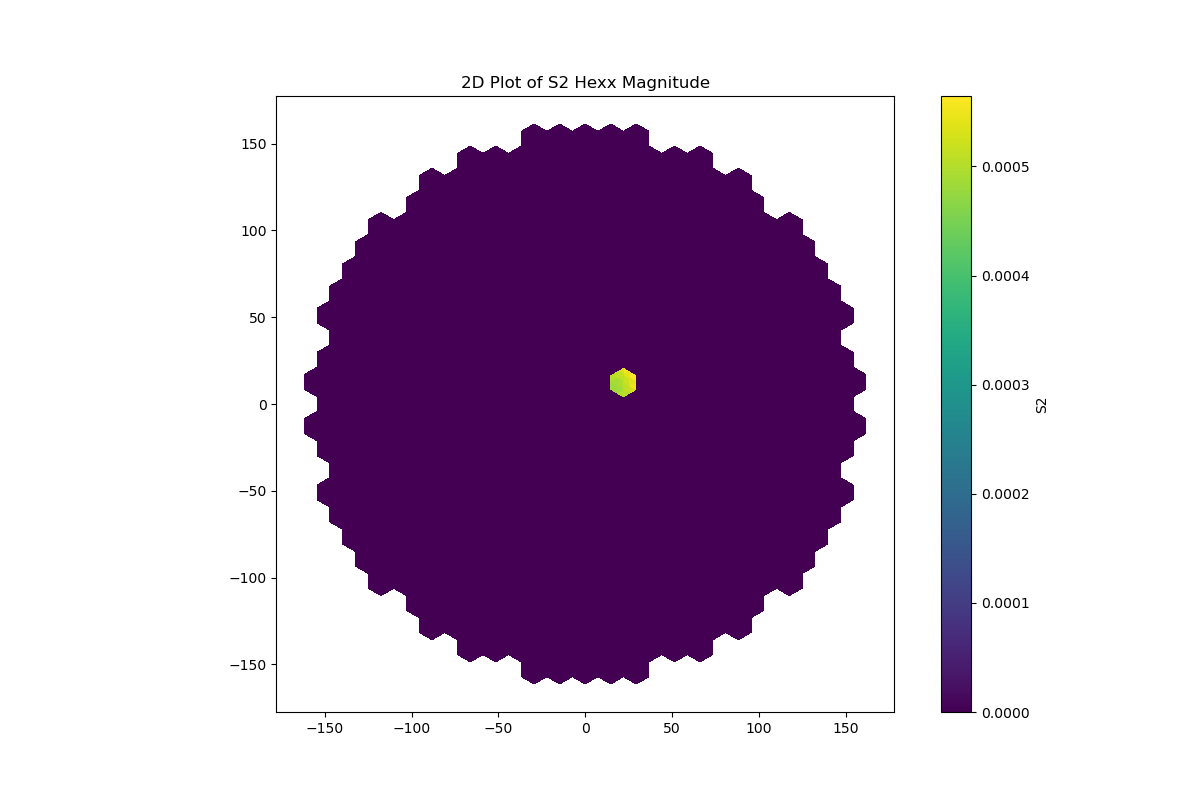
\includegraphics[width=\linewidth]{figures/OBJECTIVES1_TEST05_2DTriMG_VVER400_VandV_level2_NOISE_S_magnitude_G2.png}
        \end{subfigure}
        \caption{Noise source location for 2D VVER-400}
        \label{fig:2DVVER_source}
\end{figure}
The simulation is done at frequency of 1 Hz. There is no comparison for this simulation. The results of neutron noise simulations are described in Figure 

\begin{figure}[H]
        \centering
        \begin{subfigure}{.48\textwidth}
          \centering
          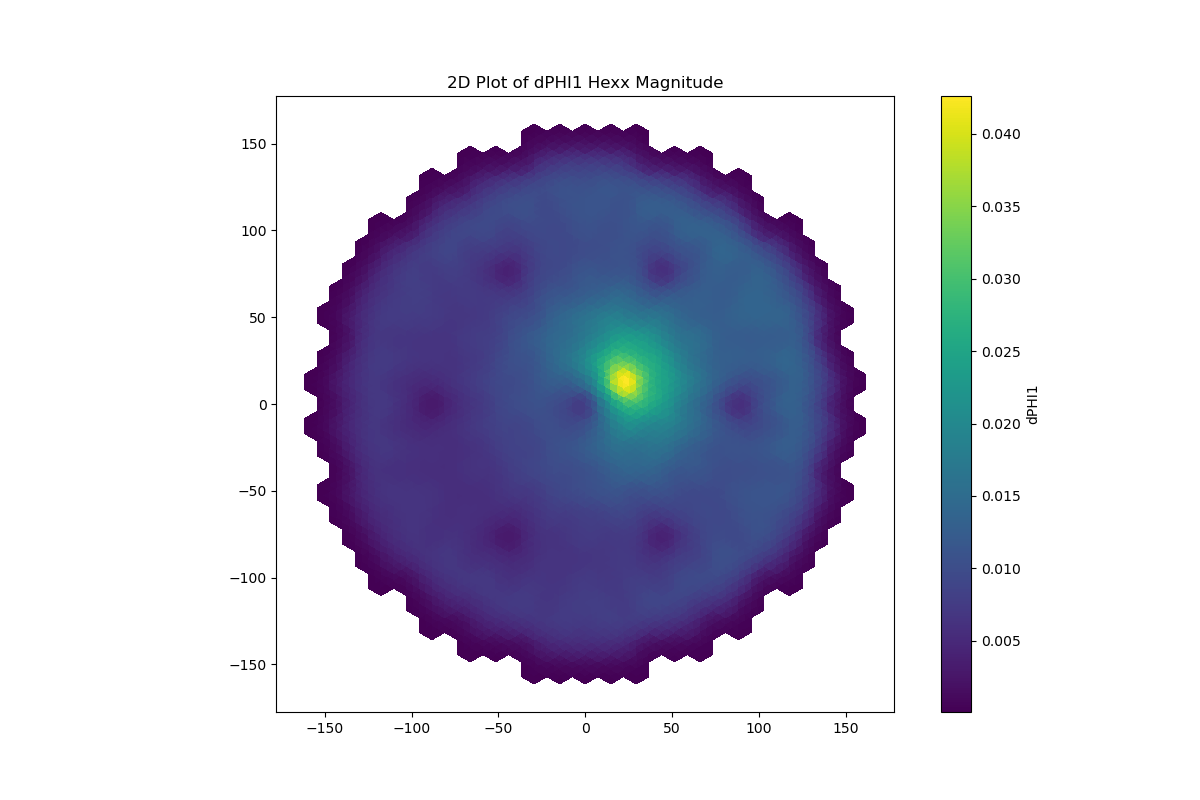
\includegraphics[width=\linewidth]{figures/OBJECTIVES1_TEST05_2DTriMG_VVER400_VandV_level2_NOISE_dPHI_magnitude_G1.png}
        \end{subfigure}
        \hfill
        \begin{subfigure}{.48\textwidth}
          \centering
          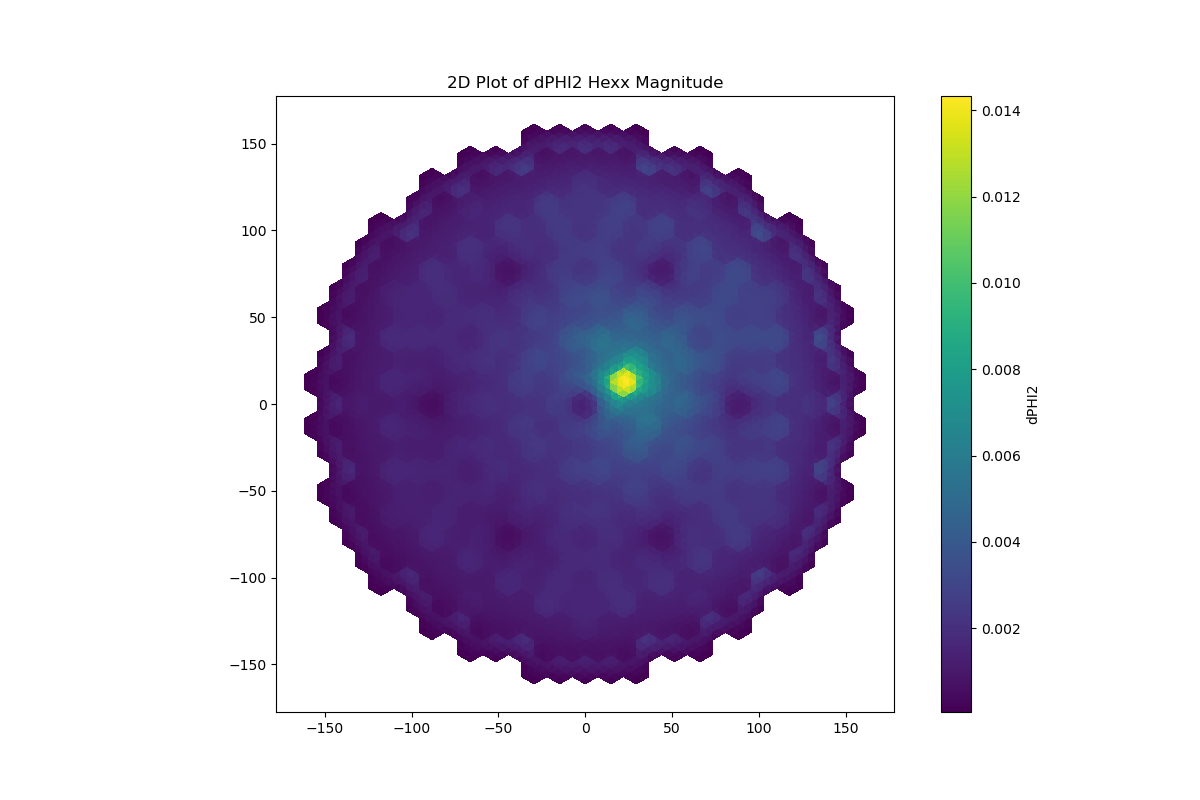
\includegraphics[width=\linewidth]{figures/OBJECTIVES1_TEST05_2DTriMG_VVER400_VandV_level2_NOISE_dPHI_magnitude_G2.png}
        \end{subfigure}
\end{figure}
\begin{figure}[H]\ContinuedFloat
        \centering
        \begin{subfigure}{.48\textwidth}
          \centering
          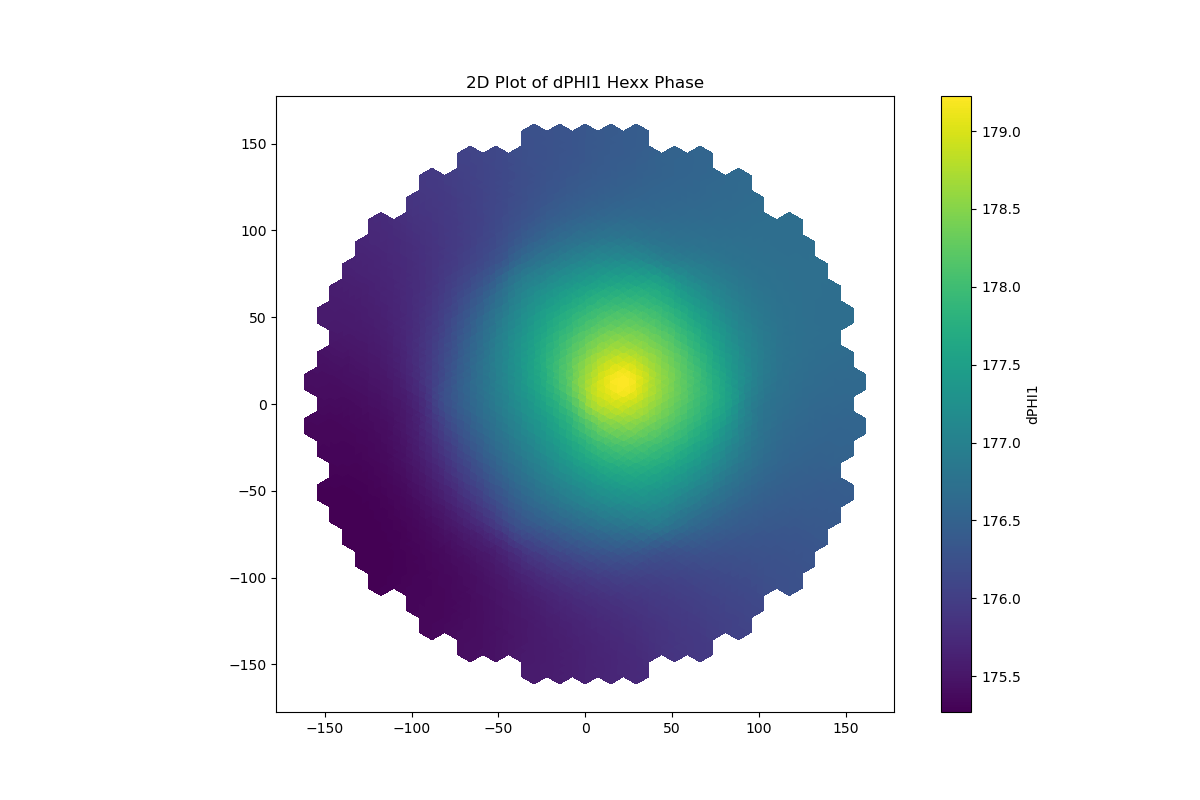
\includegraphics[width=\linewidth]{figures/OBJECTIVES1_TEST05_2DTriMG_VVER400_VandV_level2_NOISE_dPHI_phase_G1.png}
        \end{subfigure}
        \hfill
        \begin{subfigure}{.48\textwidth}
          \centering
          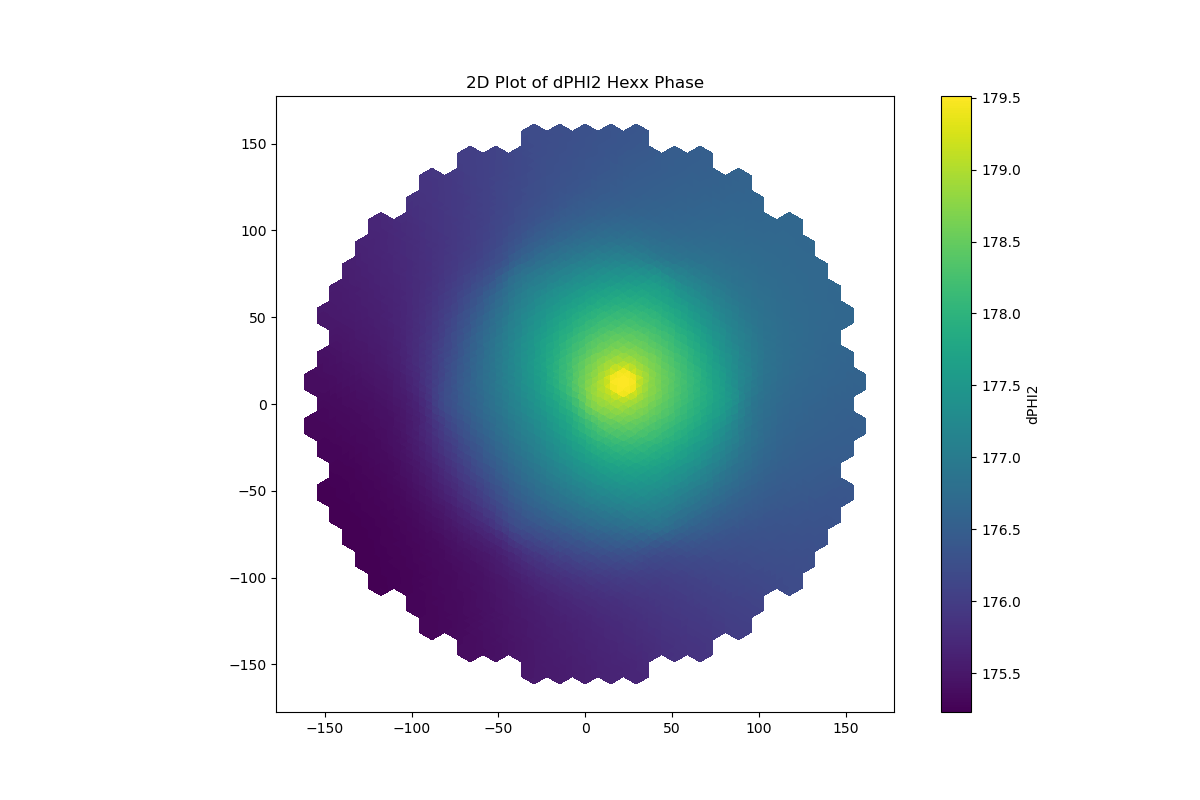
\includegraphics[width=\linewidth]{figures/OBJECTIVES1_TEST05_2DTriMG_VVER400_VandV_level2_NOISE_dPHI_phase_G2.png}
        \end{subfigure}
        \caption{Neutron noise results from the developed tool}
        \label{fig:2DVVER_noise_results}
\end{figure}

The results show that magnitude of the peak fast neutron noise is larger than the thermal neutron noise. However, the fast neutron noise is more dispersed than the thermal neutron noise. The phase plot shows similarities between fast and thermal group.

\section{3D Langenbuch (LMW) Benchmark}

\subsection{Forward Simulation}

The LMW Benchmark is a two-group, six-delayed neutron precursor families and 3D time-dependent reactor benchmark without thermal-hydraulic feedback. The reactor was developed and studied by \cite{langenbuchCoarseMeshFluxExpansionMethod1977}. The reactor consists of 77 fuel assembly 40 reflector assemblies. The size of each assembly is 20 cm $\times$ 20 cm. The zero flux boundary condition is used in this case. This case has been used to verify transient solvers due to its fast resolution \cite{vidal-ferrandizFEMFFUSIONFiniteElement2023}. The core configuration and the material cross sections are defined in Figure \ref{fig:3DLangenbuch}, Table \ref{table:3DLangenbuchXS}, and Table \ref{table:3DLangenbuchKin}. 

\begin{figure}[H]
        \centering
        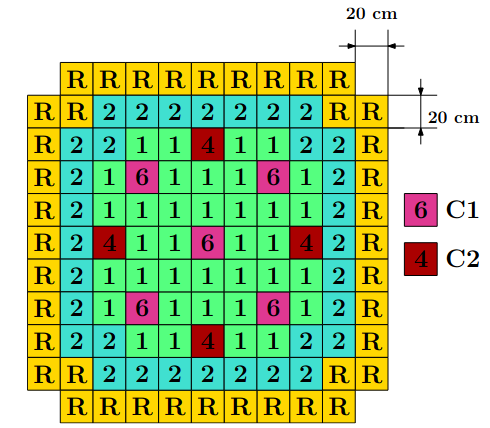
\includegraphics[width=0.45\textwidth]{figures/3DLangenbuch.png}
        \caption{Core configuration of 3D Langenbuch Benchmark (obtained from \cite{vidal-ferrandizFEMFFUSIONFiniteElement2023})}
        \label{fig:3DLangenbuch}
\end{figure}

\begin{table}[H]
        \centering
        \caption{Homogenized cross-section of 3D Langenbuch Benchmark (obtained from \cite{vidal-ferrandizFEMFFUSIONFiniteElement2023})}
        \label{table:3DLangenbuchXS}
        \begin{tabular}{ | M{4.5cm} | M{1cm} | M{1.5cm} | M{2cm} | M{2cm} | M{2cm} | } 
         \hline
         \textbf{Material} & \textbf{Group} & \textbf{$D_g$} ($cm$) & \textbf{$\Sigma_{a,g}$} ($cm^{-1}$) & \textbf{$\nu \Sigma_{f,g}$}  ($cm^{-1}$) & \textbf{$\Sigma_{s,1 \rightarrow}$}  ($cm^{-1}$)\\
         \hline
         \multirow{2}{*}{1 - Fuel} & 1 & 1.423913 & 0.010402060 & 0.006477691 & \\
         \cline{2-6}               & 2 & 0.356306 & 0.087662170 & 0.112732800 & 0.01755550 \\
         \hline
         \multirow{2}{*}{2 - Fuel} & 1 & 1.425611 & 0.010992630 & 0.007503284 & \\
         \cline{2-6}               & 2 & 0.350574 & 0.099256340 & 0.137800400 & 0.01717768 \\
         \hline
         \multirow{2}{*}{R - Reflector} & 1 & 1.634227 & 0.002660573 & 0.000000000 & \\
         \cline{2-6}                    & 2 & 0.264002 & 0.049363510 & 0.000000000 & 0.02759693 \\
         \hline
         \multirow{2}{*}{4 \& 6 - Absorbent} & 1 & 1.423913 & 0.010952060 & 0.006477691 & \\
         \cline{2-6}                         & 2 & 0.356306 & 0.091462170 & 0.112732800 & 0.01755550 \\
         \hline
         \multirow{2}{*}{5 - Reflector + Absorbent} & 1 & 1.634227 & 0.00321020 & 0.000000000 & \\
         \cline{2-6}                                & 2 & 0.264002 & 0.05316351 & 0.000000000 & 0.02759693 \\
         \hline
        \end{tabular}
\end{table}

\begin{table}[H]
        \centering
        \caption{Neutron precursors data of 3D Langenbuch Benchmark (obtained from \cite{vidal-ferrandizFEMFFUSIONFiniteElement2023})}
        \label{table:3DLangenbuchKin}
        \begin{tabular}{ | M{2.5cm} | M{1.5cm} | M{1.5cm} | M{1.5cm} | M{1.5cm} | M{1.5cm} |  M{1.5cm} |} 
         \hline
         \textbf{Group (k)} & \textbf{1} & \textbf{2} & \textbf{3} & \textbf{4} & \textbf{5} & \textbf{6} \\
         \hline
         $\beta_k$                & 0.000247 & 0.0013845 & 0.001222 & 0.0026455 & 0.000832 & 0.000169 \\
         \hline
         $\lambda_k^d$ ($s^{-1}$) & 0.0127 & 0.0317 & 0.115 & 0.311 & 1.4 & 3.87 \\
         \hline
        \end{tabular}
\end{table}

The forward simulation of the 3D Langenbuch Benchmark has been simulated in FEMFFUSION \cite{vidal-ferrandizFEMFFUSIONFiniteElement2023} and compared with the developed solver. The results are as follows:

\begin{table}[H]
        \centering
        \caption{Eigenvalue results of 3D Langenbuch (LMW) Benchmark}
        \label{table:LMW_fw_results}
        \begin{tabular}{ | M{3.5cm} | M{2cm} | } 
         \hline
         $k_{\text{eff}}$ FEMFFUSION & 0.999748   \\
         \hline
         $k_{\text{eff}}$ solver & 1.000866  \\
         \hline
         Absolute Error (pcm) & 111.8  \\
         \hline
        \end{tabular}
\end{table}

\begin{figure}[H]
        \centering
        \begin{subfigure}{.48\textwidth}
          \centering
          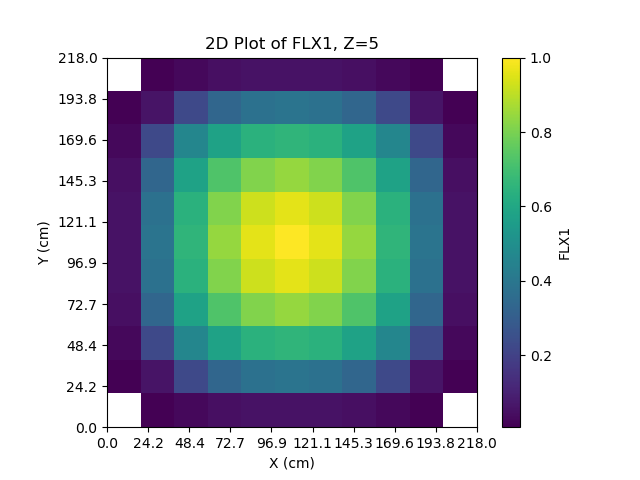
\includegraphics[width=\linewidth]{figures/OBJECTIVES1_TEST10_3DMG_Langenbuch_FORWARD_FLX_G1_Z5.png}
        \end{subfigure}
        \hfill
        \begin{subfigure}{.48\textwidth}
          \centering
          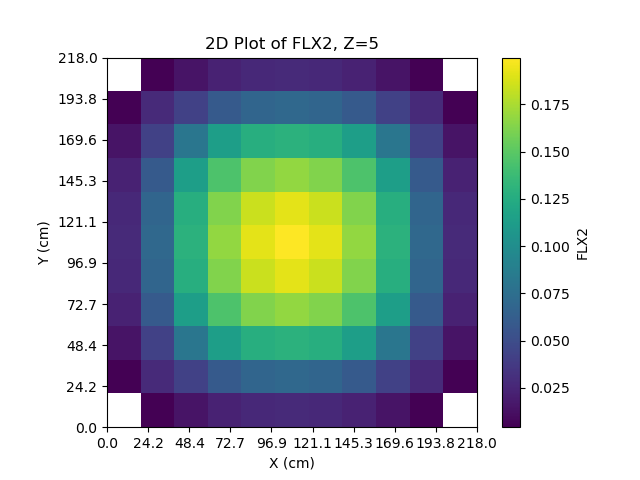
\includegraphics[width=\linewidth]{figures/OBJECTIVES1_TEST10_3DMG_Langenbuch_FORWARD_FLX_G2_Z5.png}
        \end{subfigure}
        \caption{Forward flux results from FEMFFUSION at midplane (Z=5)}
        \label{fig:LMW_fw_results_flx}
\end{figure}
\begin{figure}[H]
        \centering
        \begin{subfigure}{.48\textwidth}
          \centering
          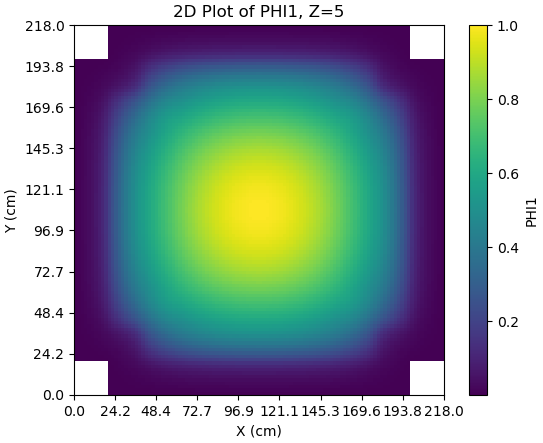
\includegraphics[width=\linewidth]{figures/OBJECTIVES1_TEST10_3DMG_Langenbuch_FORWARD_PHI_magnitude_G1_Z5.png}
        \end{subfigure}
        \hfill
        \begin{subfigure}{.48\textwidth}
          \centering
          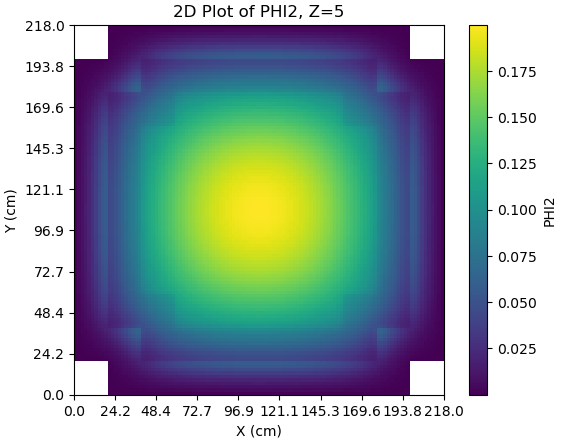
\includegraphics[width=\linewidth]{figures/OBJECTIVES1_TEST10_3DMG_Langenbuch_FORWARD_PHI_magnitude_G2_Z5.png}
        \end{subfigure}
        \caption{Forward flux results from the developed solver at midplane (Z=5)}
        \label{fig:LMW_fw_results_phi}
\end{figure}
\begin{figure}[H]
        \centering
        \begin{subfigure}{.48\textwidth}
          \centering
          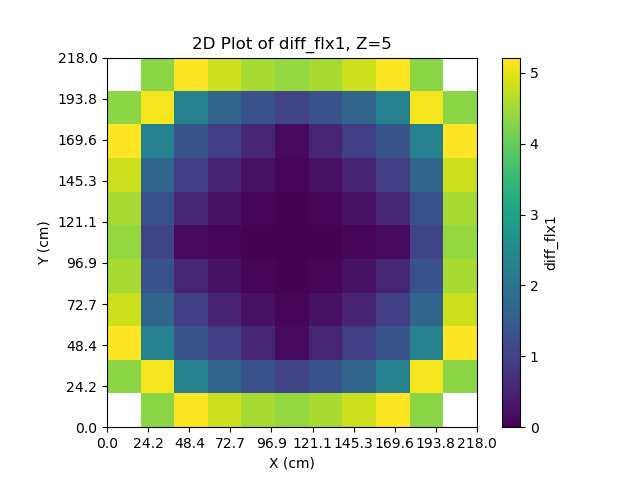
\includegraphics[width=\linewidth]{figures/OBJECTIVES1_TEST10_3DMG_Langenbuch_FORWARD_diff_flx_G1_Z5.png}
        \end{subfigure}
        \hfill
        \begin{subfigure}{.48\textwidth}
          \centering
          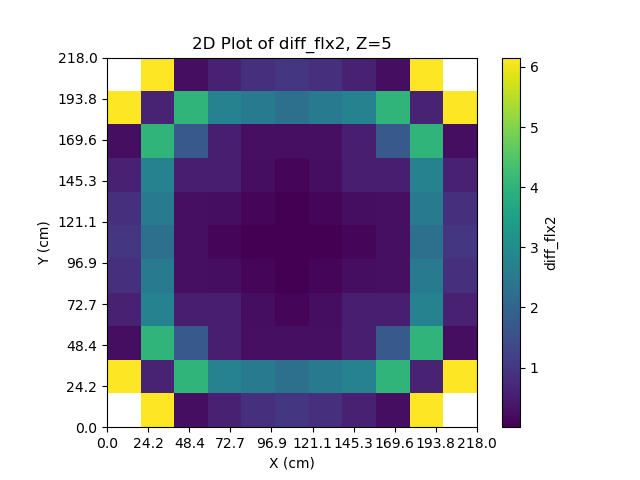
\includegraphics[width=\linewidth]{figures/OBJECTIVES1_TEST10_3DMG_Langenbuch_FORWARD_diff_flx_G2_Z5.png}
        \end{subfigure}
        \caption{Difference of forward flux between FEMFFUSION and the solver at midplane (Z=5)}
\end{figure}

The forward results show that some discrepancies are observed between the developed solver and FEMFFUSION. The difference in $k_\text{eff}$ is 111.8 pcm and the maximum error of forward flux at midplane is about 6\%. This difference is due to the use of the finite element method in FEMFFUSION, which has different degrees of accuracy compared to the box-scheme finite difference used in the solver. Considering this difference in spatial discretization method, the solver generally works well and in a certain degree of agreement with FEMFFUSION.

\subsection{Neutron Noise Simulation}

For the neutron noise simulation, the noise source is defined as an AVS-type noise source location $\textbf{r}_p$ is at the center of the core and midplane ($Z=5$). The noise sources are defined as follows:
\begin{equation}
    \begin{aligned}
        \delta \Sigma_{t,2} (\textbf{r}_p, \omega) &= 0.05 \Sigma_{t,2} (\textbf{r}_p)\\    
    \end{aligned}
\end{equation}

There is no comparison for this simulation. The results of the simulations at the midplane are described in Figure \ref{fig:Langenbuch_noise_results}.
\newpage
\begin{figure}[H]
        \centering
        \begin{subfigure}{.48\textwidth}
          \centering
          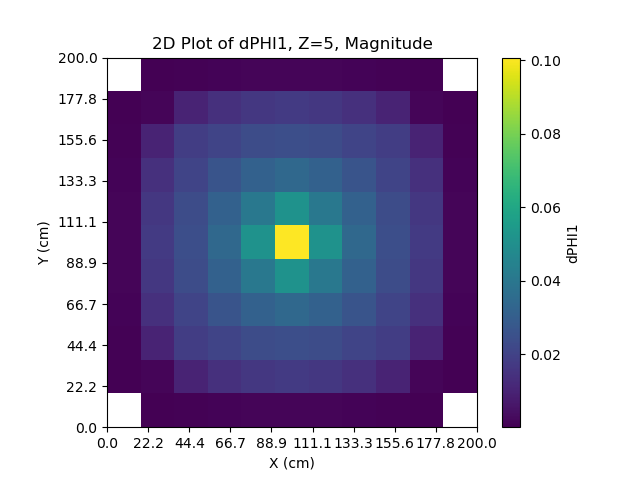
\includegraphics[width=\linewidth]{figures/OBJECTIVES1_TEST10_3DMG_Langenbuch_NOISE_dPHI_magnitude_G1_Z5.png}
        \end{subfigure}
        \hfill
        \begin{subfigure}{.48\textwidth}
          \centering
          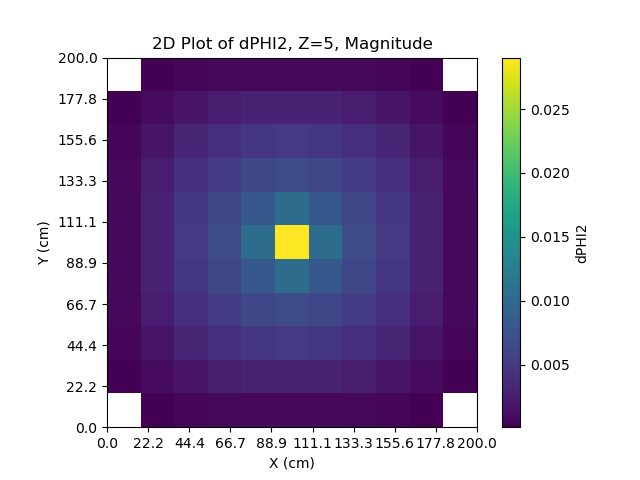
\includegraphics[width=\linewidth]{figures/OBJECTIVES1_TEST10_3DMG_Langenbuch_NOISE_dPHI_magnitude_G2_Z5.png}
        \end{subfigure}
\end{figure}
\begin{figure}[H]\ContinuedFloat
        \centering
        \begin{subfigure}{.48\textwidth}
          \centering
          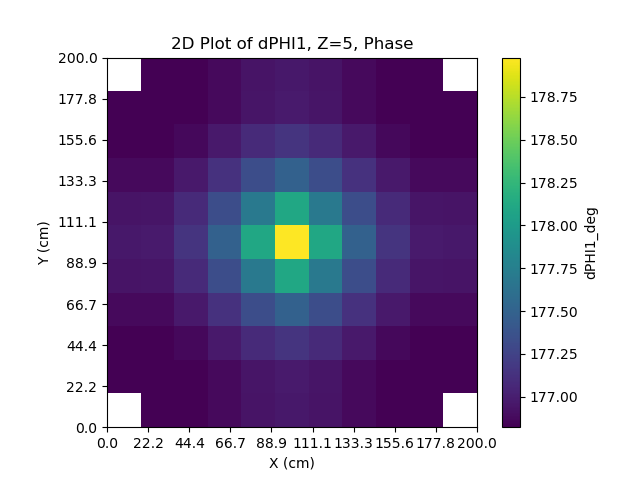
\includegraphics[width=\linewidth]{figures/OBJECTIVES1_TEST10_3DMG_Langenbuch_NOISE_dPHI_phase_G1_Z5.png}
        \end{subfigure}
        \hfill
        \begin{subfigure}{.48\textwidth}
          \centering
          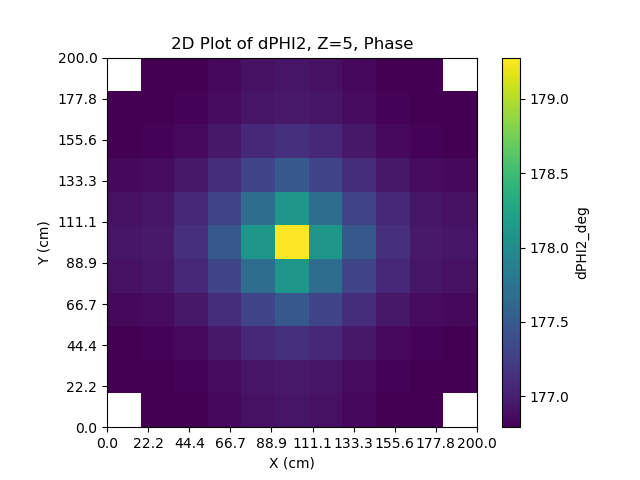
\includegraphics[width=\linewidth]{figures/OBJECTIVES1_TEST10_3DMG_Langenbuch_NOISE_dPHI_phase_G2_Z5.png}
        \end{subfigure}
        \caption{Neutron noise results from the developed solver}
        \label{fig:Langenbuch_noise_results}
\end{figure}

The results show that magnitude of the peak fast neutron noise is larger than the thermal neutron noise. However, the fast neutron noise is more dispersed than the thermal neutron noise. The phase plot shows similarities between fast and thermal group.

\section{3D VVER-400}

\subsection{Forward Simulation}

Water-Water energetic reactor (VVER) is a pressurized water reactor with a possible delivery design of 440 MW among others. This benchmark corresponds to an asymmetric control rod ejection accident in a VVER-440 core. However, only steady-state forward flux simulation is done in this case. The radial and axial configuration of the core is shown in Figure \ref{fig:3DVVER400}, and the homogenized cross-section data is shown in Table \ref{table:3DVVER400XS}. The active core height is 250 cm with 12 planes of assemblies across the core. The data reference of 3D-VVER440 benchmark problem are extracted from \cite{chaoConformalMappingHexagonal1995}.

\begin{figure}[H]
        \centering
        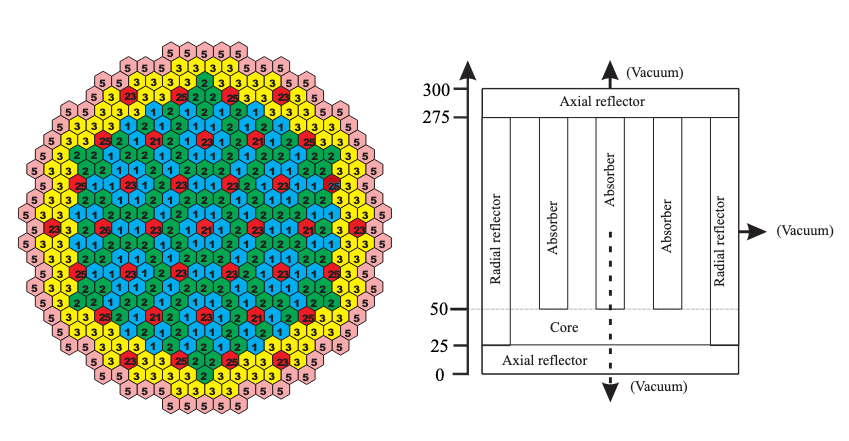
\includegraphics[width=0.7\textwidth]{figures/3DVVER400.png}
        \caption{Core configuration of 3D VVER-400 (obtained from \cite{vidal-ferrandizFEMFFUSIONFiniteElement2023})}
        \label{fig:3DVVER400}
\end{figure}

\begin{table}[H]
        \centering
        \caption{Homogenized cross-section and neutron precursors data of 3D VVER-400 (obtained from \cite{vidal-ferrandizFEMFFUSIONFiniteElement2023})}
        \label{table:3DVVER400XS}
        \begin{tabular}{ | M{4.5cm} | M{1cm} | M{2cm} | M{2cm} | M{2cm} | M{2cm} | } 
         \hline
         \textbf{Material} & \textbf{Group} & \textbf{$D_g$} ($cm$) & \textbf{$\Sigma_{t,g}$} ($cm^{-1}$) & \textbf{$\nu \Sigma_{f,g}$}  ($cm^{-1}$) & \textbf{$\Sigma_{s,1 \rightarrow}$}  ($cm^{-1}$)\\
         \hline
         \multirow{2}{*}{1 - Fuel} & 1 & 1.34660E+00 & 2.52550E-02 & 4.44880E-03 & \\
         \cline{2-6}               & 2 & 3.71690E-01 & 6.42770E-02 & 7.37530E-02 & 1.68930E-02  \\
         \hline
         \multirow{2}{*}{2 - Fuel} & 1 & 1.33770E+00 & 2.47090E-02 & 5.53370E-03 & \\
         \cline{2-6}               & 2 & 3.69180E-01 & 7.93610E-02 & 1.05810E-01 & 1.59120E-02 \\
         \hline
         \multirow{2}{*}{3 - Fuel} & 1 & 1.33220E+00 & 2.43500E-02  & 7.03910E-03 & \\
         \cline{2-6}               & 2 & 3.65020E-01 & 1.00100E-01  & 1.49640E-01 & 1.48880E-02 \\
         \hline
         \multirow{2}{*}{4 - Absorber} & 1 & 1.19530E+00 & 3.56360E-02 & 0.00000E+00 & \\
         \cline{2-6}                   & 2 & 1.93130E-01 & 1.34980E-01 & 0.00000E+00 & 2.22640E-02 \\
         \hline
         \multirow{2}{*}{5 - Radial Reflector} & 1 & 1.44850E+00 & 3.31840E-02 & 0.00000E+00 & \\
         \cline{2-6}                           & 2 & 2.51760E-01 & 3.28390E-02 & 0.00000E+00 & 3.22620E-02 \\
         \hline
         \multirow{2}{*}{6 - Axial Reflector} & 1 & 1.34130E+00 & 2.93010E-02 & 0.00000E+00 & \\
         \cline{2-6}                          & 2 & 2.48710E-01 & 6.46550E-02 & 0.00000E+00 & 2.71480E-02 \\
         \hline
        \end{tabular}
\end{table}

The forward simulation of the 3D VVER-400 has been simulated in FEMFFUSION \cite{vidal-ferrandizFEMFFUSIONFiniteElement2023} and compared with the developed solver. The results are as follows:

\begin{table}[H]
        \centering
        \caption{Eigenvalue results of 3D VVER-400}
        \label{table:3DVVER_fw_results}
        \begin{tabular}{ | M{3.5cm} | M{2cm} | } 
         \hline
         $k_{\text{eff}}$ FEMFFUSION & 1.002440   \\
         \hline
         $k_{\text{eff}}$ solver & 1.003326  \\
         \hline
         Absolute Error (pcm) & 88.6  \\
         \hline
        \end{tabular}
\end{table}

\begin{figure}[H]
        \centering
        \begin{subfigure}{.48\textwidth}
          \centering
          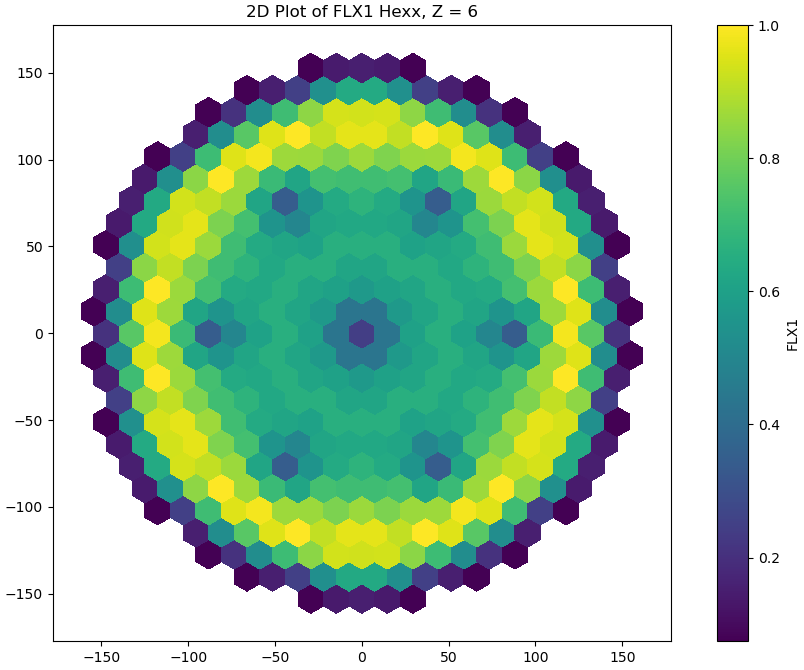
\includegraphics[width=\linewidth]{figures/OBJECTIVES1_TEST07_3DTriMG_VVER400_VandV_level2_FORWARD_FLX_magnitude_G1_Z6.png}
        \end{subfigure}
        \hfill
        \begin{subfigure}{.48\textwidth}
          \centering
          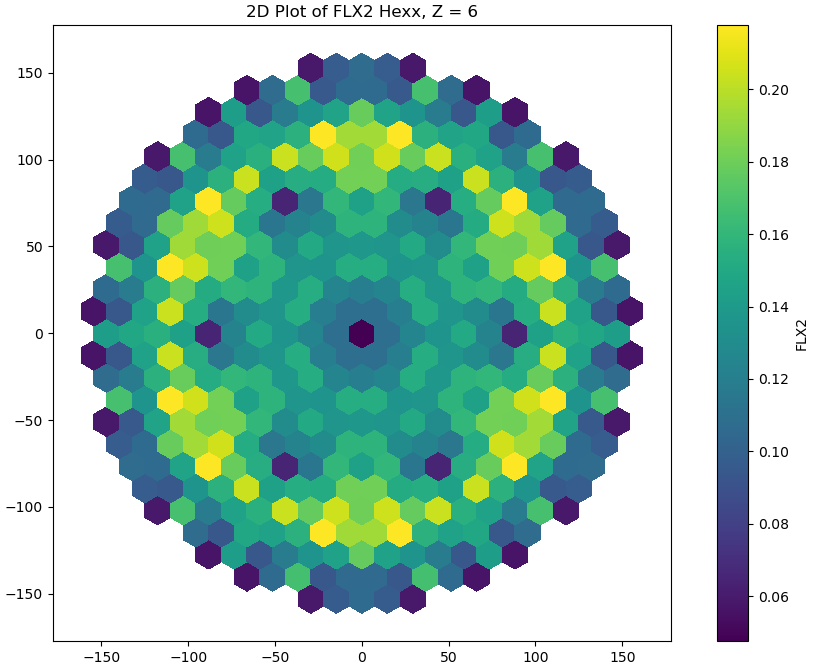
\includegraphics[width=\linewidth]{figures/OBJECTIVES1_TEST07_3DTriMG_VVER400_VandV_level2_FORWARD_FLX_magnitude_G2_Z6.png}
        \end{subfigure}
        \caption{Forward flux results from FEMFFUSION at midplane (Z=6)}
        \label{fig:3DVVER_fw_results_flx}
\end{figure}
\begin{figure}[H]
        \centering
        \begin{subfigure}{.48\textwidth}
          \centering
          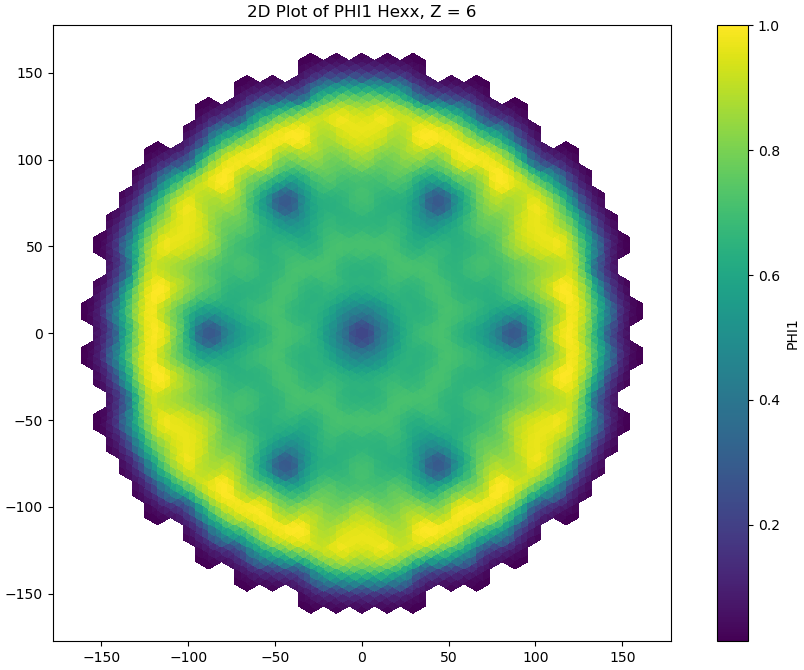
\includegraphics[width=\linewidth]{figures/OBJECTIVES1_TEST07_3DTriMG_VVER400_VandV_level2_FORWARD_PHI_magnitude_G1_Z6.png}
        \end{subfigure}
        \hfill
        \begin{subfigure}{.48\textwidth}
          \centering
          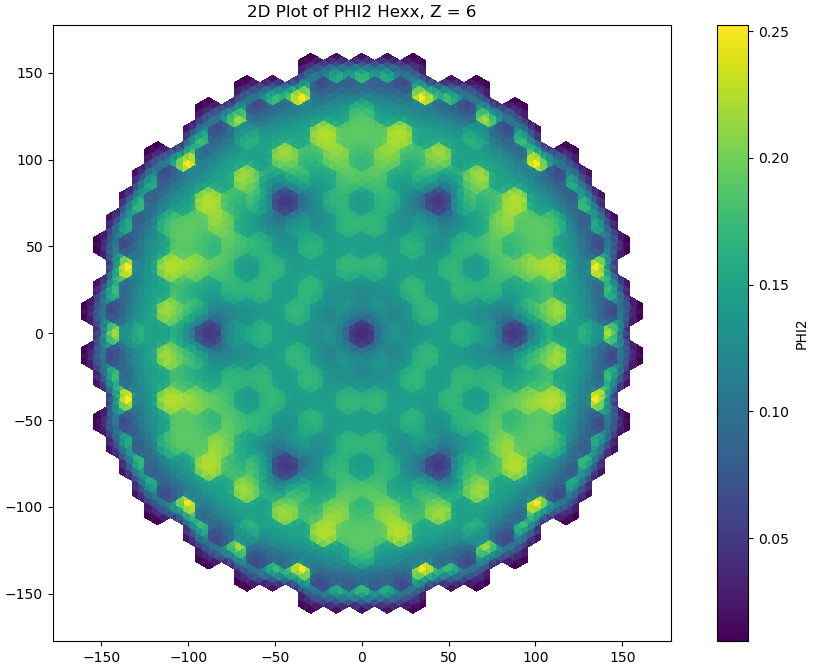
\includegraphics[width=\linewidth]{figures/OBJECTIVES1_TEST07_3DTriMG_VVER400_VandV_level2_FORWARD_PHI_magnitude_G2_Z6.png}
        \end{subfigure}
        \caption{Forward flux results from the developed solver at midplane (Z=6)}
        \label{fig:3DVVER_fw_results_phi}
\end{figure}
\begin{figure}[H]
        \centering
        \begin{subfigure}{.48\textwidth}
          \centering
          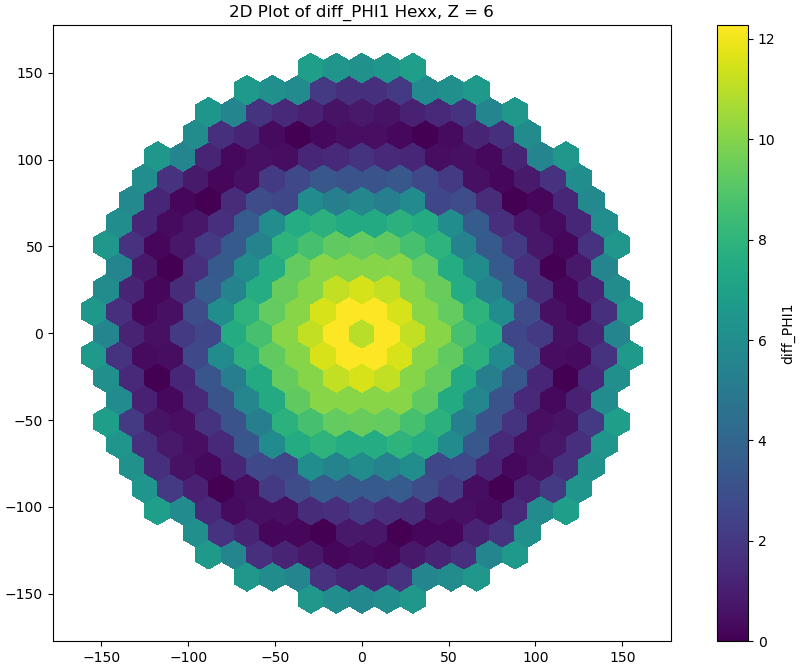
\includegraphics[width=\linewidth]{figures/OBJECTIVES1_TEST07_3DTriMG_VVER400_VandV_level2_FORWARD_diff_PHI_magnitude_G1_Z6.png}
        \end{subfigure}
        \hfill
        \begin{subfigure}{.48\textwidth}
          \centering
          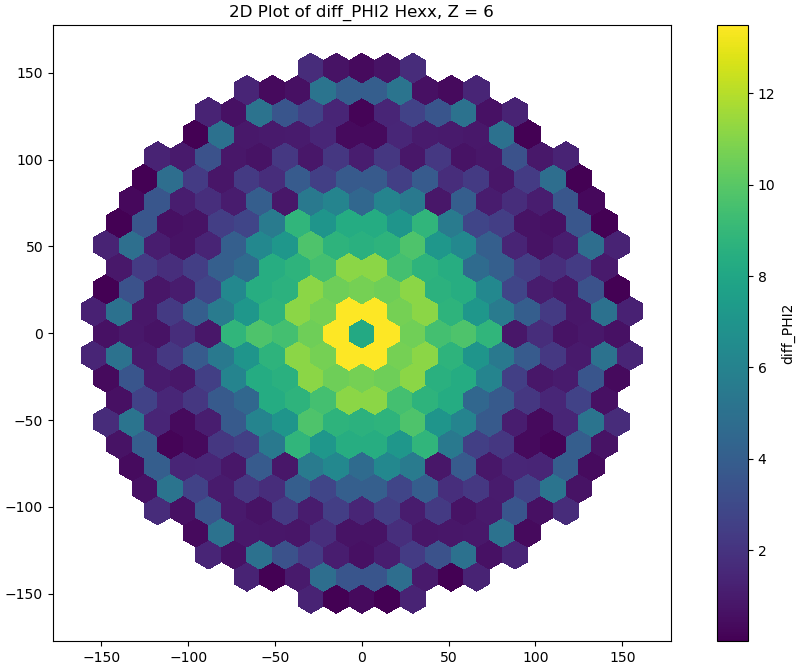
\includegraphics[width=\linewidth]{figures/OBJECTIVES1_TEST07_3DTriMG_VVER400_VandV_level2_FORWARD_diff_PHI_magnitude_G2_Z6.png}
        \end{subfigure}
        \caption{Difference of forward flux between FEMFFUSION and the solver at midplane (Z=6)}
\end{figure}

The forward results show that some discrepancies are observed between the developed solver and FEMFFUSION. The difference in $k_\text{eff}$ is 88.6 pcm and the maximum error of forward flux at midplane is about 12\%. This difference is due to the use of the finite element method in FEMFFUSION, which has different degrees of accuracy compared to the box-scheme finite difference used in the solver. Considering this difference in spatial discretization method, the solver generally works well and in a certain degree of agreement with FEMFFUSION.

\subsection{Neutron Noise Simulation}

For the neutron noise simulation, the noise source is defined as an AVS-type noise source location $\textbf{r}_p$ is near the center of the core and midplane ($Z=7$), indicated by yellow hexagon in Figure \ref{fig:3DVVER_source}. The noise sources are defined as follows:
\begin{equation}
    \begin{aligned}
        \delta \Sigma_{t,2} (\textbf{r}_p, \omega) &= 0.05 \Sigma_{t,2} (\textbf{r}_p)\\    
    \end{aligned}
\end{equation}

\begin{figure}[H]
        \centering
        \begin{subfigure}{.48\textwidth}
          \centering
          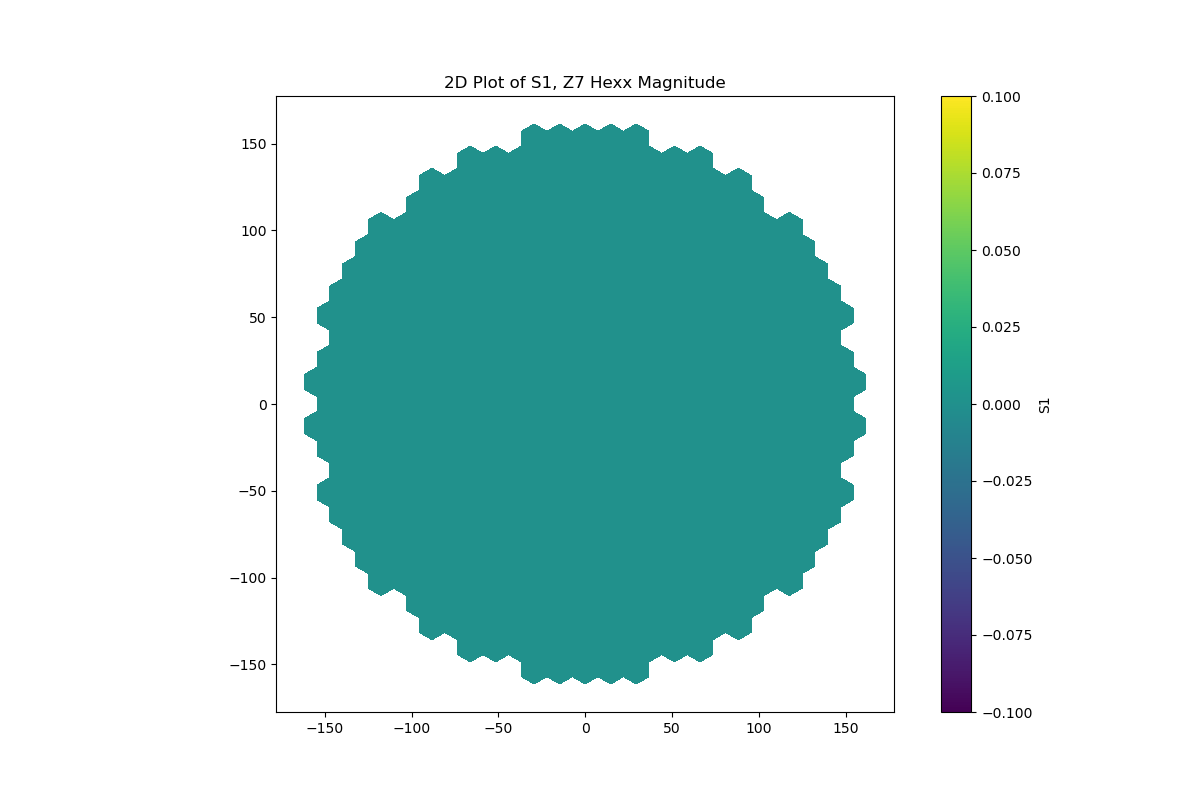
\includegraphics[width=\linewidth]{figures/OBJECTIVES1_TEST07_3DTriMG_VVER400_VandV_level2_NOISE_S_magnitude_G1_Z7.png}
        \end{subfigure}
        \hfill
        \begin{subfigure}{.48\textwidth}
          \centering
          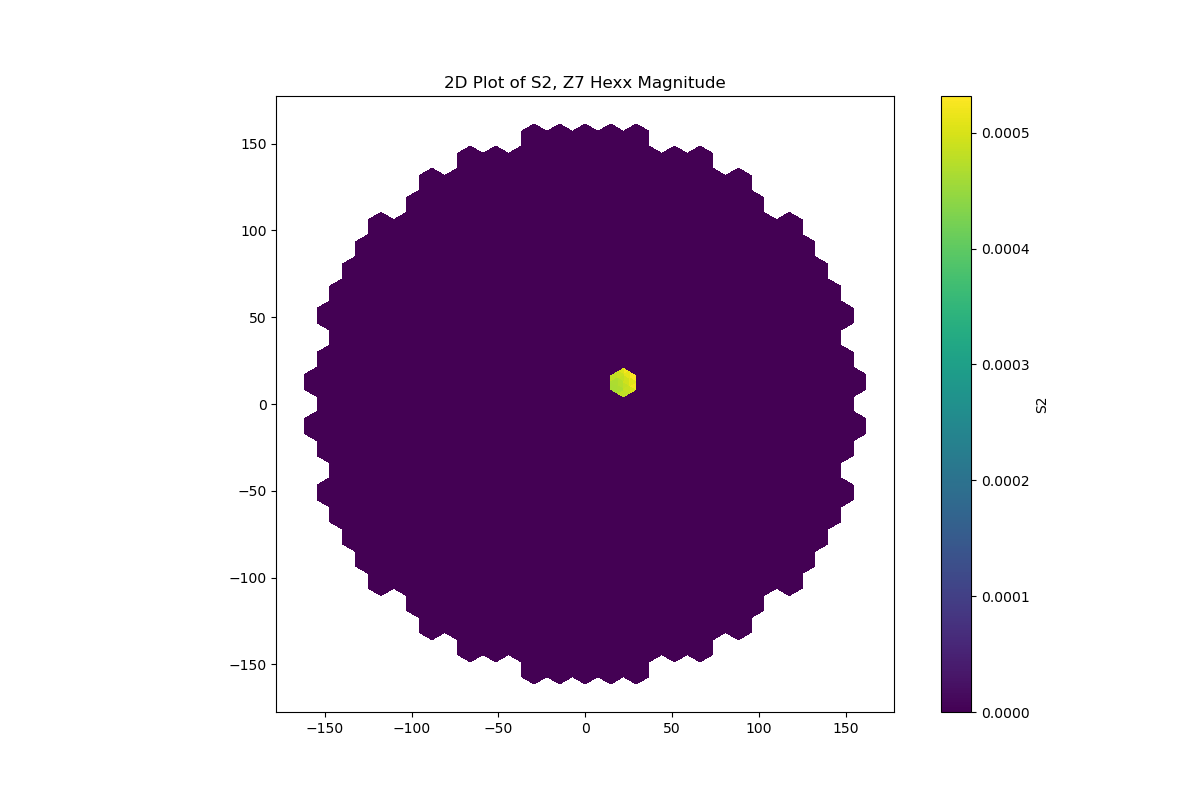
\includegraphics[width=\linewidth]{figures/OBJECTIVES1_TEST07_3DTriMG_VVER400_VandV_level2_NOISE_S_magnitude_G2_Z7.png}
        \end{subfigure}
        \caption{Noise source location for 3D VVER-400}
        \label{fig:3DVVER_source}
\end{figure}

There is no comparison for this simulation. The results of the simulations at the midplane are described in Figure \ref{fig:3DVVER_noise_results}.
\begin{figure}[H]
        \centering
        \begin{subfigure}{.48\textwidth}
          \centering
          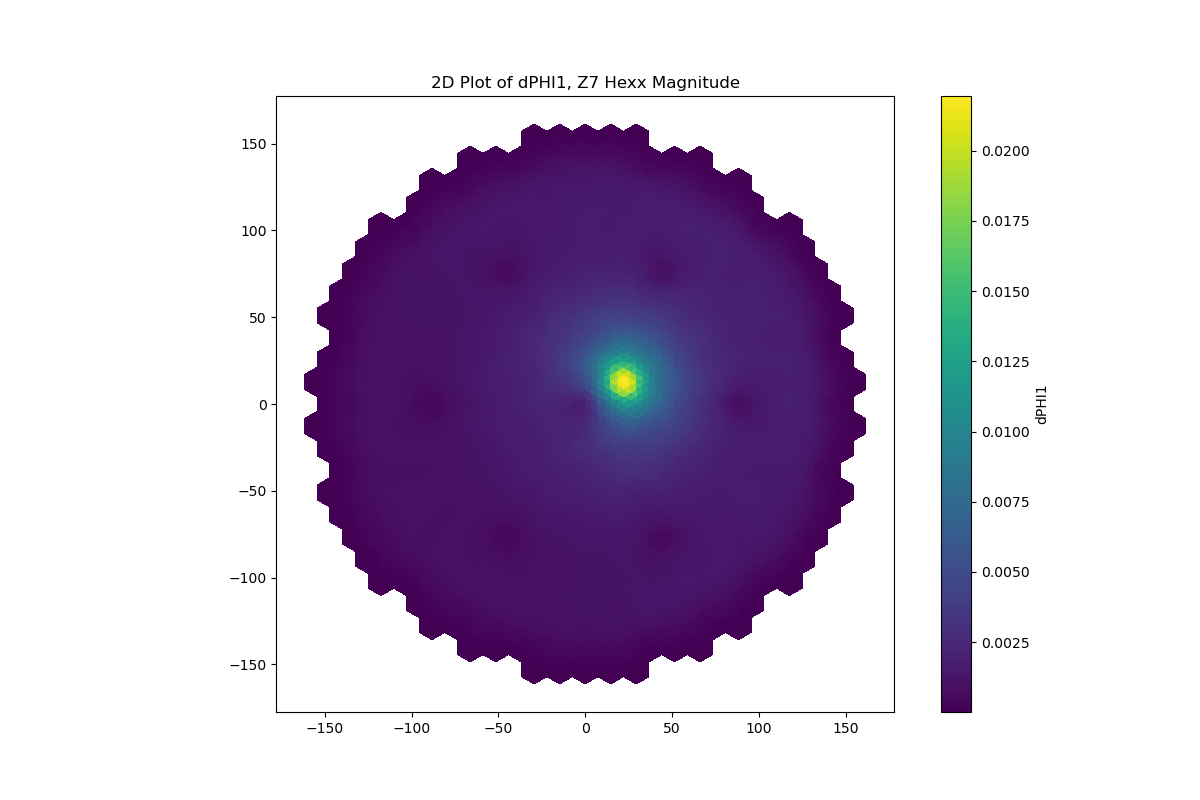
\includegraphics[width=\linewidth]{figures/OBJECTIVES1_TEST07_3DTriMG_VVER400_VandV_level2_NOISE_dPHI_magnitude_G1_Z7.png}
        \end{subfigure}
        \hfill
        \begin{subfigure}{.48\textwidth}
          \centering
          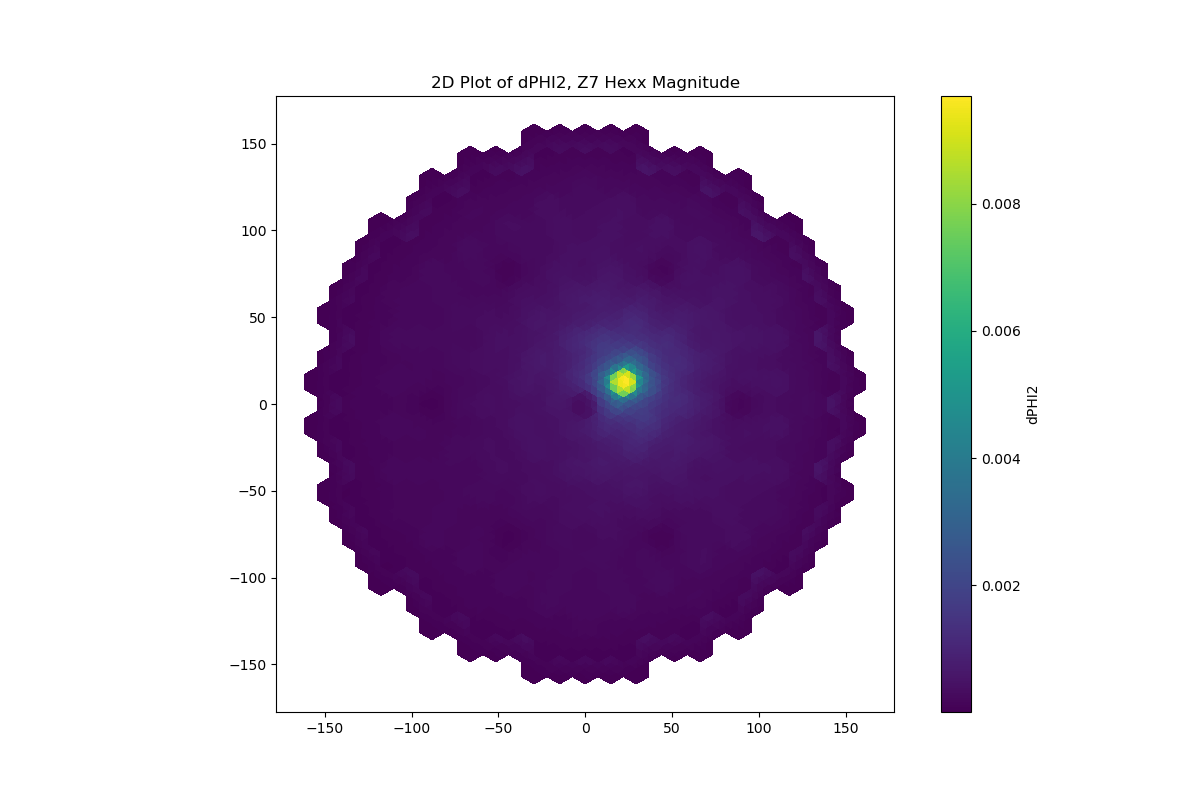
\includegraphics[width=\linewidth]{figures/OBJECTIVES1_TEST07_3DTriMG_VVER400_VandV_level2_NOISE_dPHI_magnitude_G2_Z7.png}
        \end{subfigure}
\end{figure}
\begin{figure}[H]\ContinuedFloat
        \centering
        \begin{subfigure}{.48\textwidth}
          \centering
          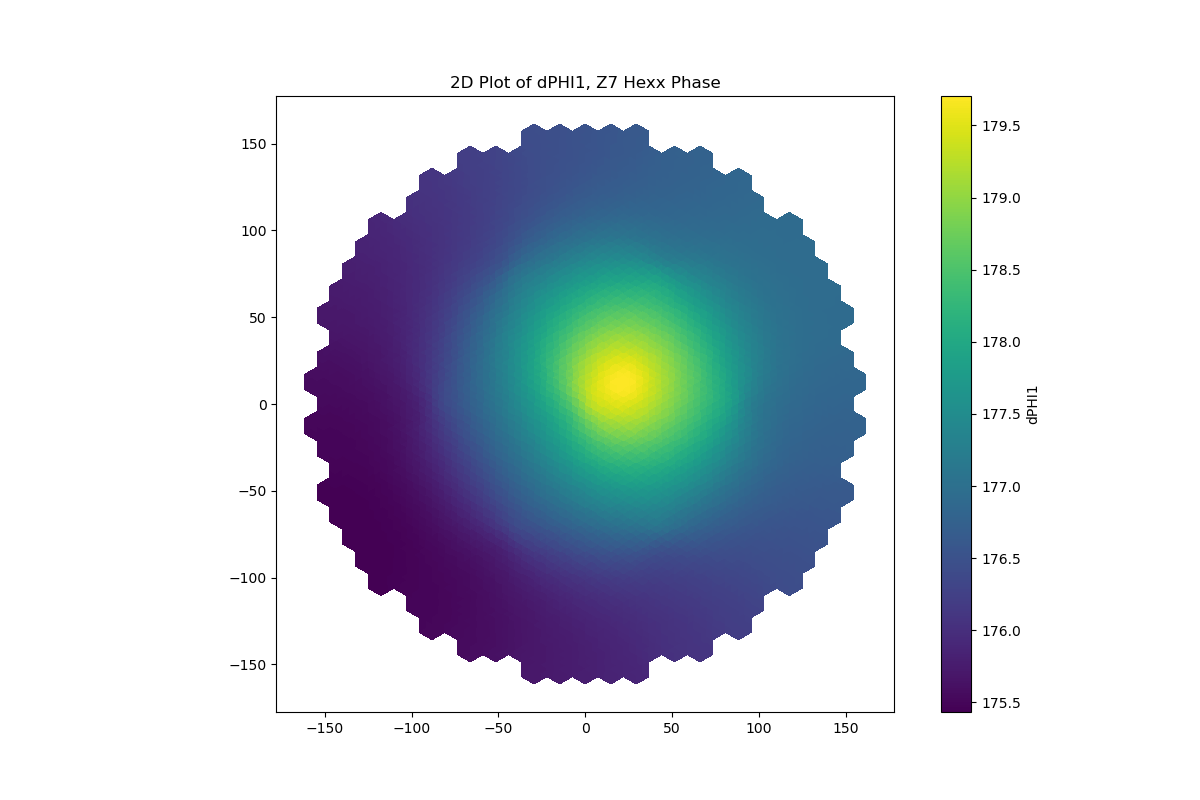
\includegraphics[width=\linewidth]{figures/OBJECTIVES1_TEST07_3DTriMG_VVER400_VandV_level2_NOISE_dPHI_phase_G1_Z7.png}
        \end{subfigure}
        \hfill
        \begin{subfigure}{.48\textwidth}
          \centering
          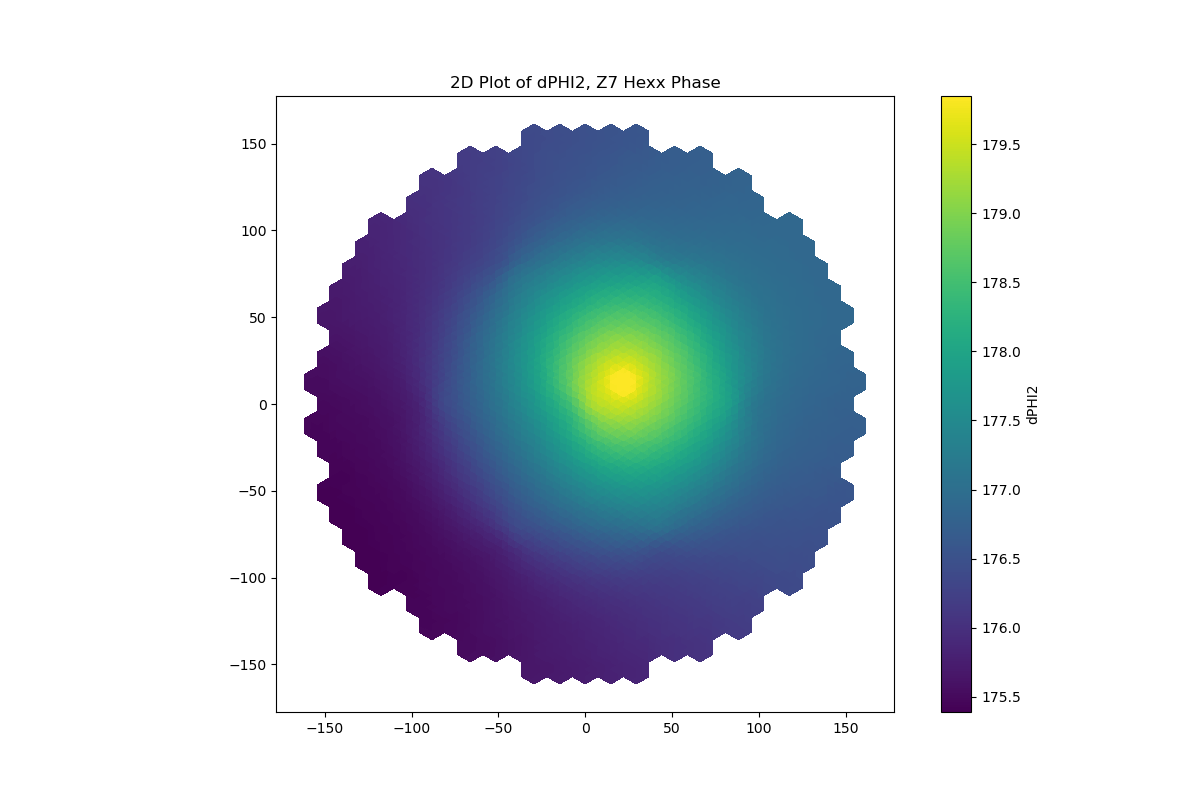
\includegraphics[width=\linewidth]{figures/OBJECTIVES1_TEST07_3DTriMG_VVER400_VandV_level2_NOISE_dPHI_phase_G2_Z7.png}
        \end{subfigure}
        \caption{Neutron noise results from the developed solver}
        \label{fig:3DVVER_noise_results}
\end{figure}

The results show that magnitude of the peak fast neutron noise is larger than the thermal neutron noise. However, the fast neutron noise is more dispersed than the thermal neutron noise. The phase plot shows similarities between fast and thermal group.
